% ==============================================================================
% PROVISIONAL — NOT CAMERA-READY
%
% Document: Adaptive Runtime Memory Governance (ARMG)
% Target Template: IEEEtran Conference (Two-Column Format)
% Note: Author block integrated per Step 6.1 specification.
%       Venue-specific IEEEtran.cls and compiler toolchain are pending final
%       conference venue identification and environment provisioning.
% ==============================================================================

\documentclass[conference]{IEEEtran}

\usepackage{amsmath,amssymb,amsfonts}
\usepackage{algorithmic}
\usepackage{graphicx}
\usepackage{textcomp}
\usepackage{xcolor}
\usepackage{booktabs}
\usepackage{cite}
\usepackage{url}
\usepackage{microtype}
\usepackage{centernot}

\graphicspath{{figures/png/}{figures/svg/}}

\begin{document}

\title{Adaptive Runtime Memory Governance: Closed-Loop Operational Knowledge Extraction, Repair Efficiency, and Execution Safety in Local Text-to-SQL Systems}

\author{
\IEEEauthorblockN{Inampudi Govardhana Rao}
\IEEEauthorblockA{
School of Computer Science and Engineering\\
Email: govardhanarao.i@vitap.ac.in
}
\and
\IEEEauthorblockN{Ghanta Sundar Siddhartha}
\IEEEauthorblockA{
B.Tech CSE Core\\
Email: siddharthaghanta10@gmail.com
}
\and
\IEEEauthorblockN{Sudarsanan Shilpa}
\IEEEauthorblockA{
B.Tech CSE Core\\
Email: shilpasudarsanan4@gmail.com
}
\and
\IEEEauthorblockN{Bommadevara S N V Datta Prasada Rayulu}
\IEEEauthorblockA{
B.Tech CSE Core\\
Email: dattabommadevara123@gmail.com
}
\and
\IEEEauthorblockN{Velpuri Danaiah}
\IEEEauthorblockA{
B.Tech CSE Core\\
Email: danaiahvelpuri78@gmail.com
}
}

\maketitle

\begin{abstract}
Deploying local Large Language Models (LLMs) for enterprise Text-to-SQL workflows introduces acute operational challenges: repetitive schema repair oscillations, unconstrained vector memory accumulation in retrieval stores, and the catastrophic risk of executing destructive SQL mutations against relational warehouses. Standard stateless self-correction prompts models with raw database errors without cross-query operational memory, while unmanaged vector retrieval systems suffer from duplicate accumulation and memory bloat. This paper presents \textbf{Adaptive Runtime Memory Governance (ARMG)}, a closed-loop runtime architecture that converts PostgreSQL database execution feedback into governed, reusable operational memory. ARMG wraps frozen local open-weights models in a 10-node directed state graph integrating deterministic Abstract Syntax Tree (AST) and catalog-based error diagnosis across a canonical 7-tier exception taxonomy, ephemeral knowledge extraction, admission- and reinforcement-gated FAISS vector memory, diagnostic negative constraints, and a deterministic pre-execution AST safety guardrail.

In an empirical evaluation across three isolated repeated benchmark executions ($n = 3$, comprising 450 total evaluated query runs across six experimental modes) on a 25-query synthetic enterprise-style Star Schema data warehouse using local \texttt{qwen2.5:7b-instruct} under greedy decoding (\texttt{temperature = 0.0}), ARMG achieved verified pre-execution safety, preventing any destructive SQL statement from reaching the PostgreSQL database. Relative to stateless self-correction, ARMG achieved an observed \textbf{34.38\% reduction in mean repair iterations} (0.28 vs. 0.43 retries per query) and a \textbf{5.30\% reduction in token consumption} (542.37 vs. 572.72 tokens per query), while increasing PostgreSQL execution success from 92.00\% to 96.00\%. Furthermore, algorithmic mutual exclusion between reinforcement and admission maintained persistent vector store size invariant at exactly 3 memories in the evaluated sequential benchmark, compared to unmanaged retrieval accumulation (23 memories). However, ARMG incurred a \textbf{19.79\% end-to-end latency overhead} (8,564.89~ms vs. 7,149.68~ms) due to embedding generation and state-graph orchestration, and \textbf{relational execution accuracy plateaued identically at 68.00\%} (17 of 25 queries) across both ARMG and stateless self-correction. In addition, continuous exponential temporal decay remained experimentally unexercised under the $\sim$3.5-minute benchmark execution clock. These findings demonstrate that governed operational memory provides bounded repair behavior, token economy, and verifiable execution safety, while establishing that operational memory alone does not resolve the baseline semantic window-function reasoning boundaries of local 7B-parameter models.
\end{abstract}

\begin{IEEEkeywords}
Text-to-SQL, Large Language Models, Runtime Memory Governance, Vector Retrieval, Database Safety, Query Repair, LangGraph, Enterprise Data Warehouses.
\end{IEEEkeywords}

\section{Introduction}
Enterprise adoption of natural language interfaces to relational databases (Text-to-SQL) has accelerated with advances in instruction-tuned Large Language Models \cite{pourreza2023dinsql, gao2024dailsql}. However, organizations subject to stringent data privacy, sovereignty, or computational cost constraints increasingly mandate on-premises deployment using localized open-weights models (e.g., 7B-parameter architectures) \cite{qwen2024qwen25}. Deploying smaller LLMs locally introduces critical operational challenges:
\begin{enumerate}
    \item \textbf{Repetitive Repair Failures}: Stateless self-correction approaches \cite{madaan2023selfrefine, shinn2023reflexion} prompt the language model with raw database driver execution exceptions. Without persistent cross-query memory, the model frequently oscillates between identical invalid SQL syntax or schema constructs across successive repair cycles.
    \item \textbf{Retrieval Corruption \& Memory Bloat}: Naive implementations of retrieval augmentation \cite{lewis2020rag} that append historical execution exemplars without explicit lifecycle governance risk accumulating duplicate, conflicting, or stale entries over time \cite{park2023generativeagents, packer2023memgpt}.
    \item \textbf{Execution Safety Hazards}: Unbounded Text-to-SQL agents risk synthesizing destructive Data Manipulation Language (DML) or Data Definition Language (DDL) statements (\texttt{DELETE}, \texttt{DROP}, \texttt{UPDATE}, \texttt{TRUNCATE}), presenting severe operational risks if connected to live warehouse environments \cite{rebedea2023nemoguardrails, mao2023sqlglot, halfond2005amnesia}.
    \item \textbf{The Executable vs. Relational Correctness Gap}: While commercial evaluations frequently report database execution rates, executable SQL is frequently non-equivalent to the analytical intent of the user \cite{finegandollak2018eval, zhong2020distilled}.
\end{enumerate}

To address these limitations, we introduce \textbf{Adaptive Runtime Memory Governance (ARMG)}, a closed-loop runtime architecture that governs the extraction, admission, retrieval, reinforcement, and application of runtime operational knowledge for local Text-to-SQL systems. Rather than updating underlying model weights via fine-tuning, ARMG structures execution feedback into an ephemeral diagnostic intermediate representation (\texttt{RuntimeKnowledge}) that undergoes mathematical admission gating before entering a persistent FAISS vector index. Crucially, ARMG enforces strict algorithmic mutual exclusion between the reinforcement of existing memories and the admission of new knowledge, preventing duplicate memory accumulation. A deterministic Abstract Syntax Tree (AST) validation layer parses every query prior to database driver invocation, halting destructive mutations before execution.

\subsection{Research Gap Formulation}
While recent research has advanced decomposed in-context learning \cite{pourreza2023dinsql}, multi-agent collaboration \cite{wang2025macsql}, and verbal self-correction \cite{madaan2023selfrefine, shinn2023reflexion}, prior work has focused primarily on cloud-hosted frontier models and single-turn query synthesis. Existing frameworks do not explicitly investigate how to maintain persistent, governed operational knowledge across sequential queries in resource-constrained local environments without inducing vector store bloat, nor do they couple execution repair with deterministic AST-level pre-execution safety barriers. \textbf{ARMG investigates an integrated runtime governance architecture combining:}
\begin{enumerate}
    \item Local open-weights Text-to-SQL inference;
    \item Runtime physical database execution feedback;
    \item Zero-token deterministic 7-tier exception diagnosis;
    \item Ephemeral intermediate knowledge representation;
    \item Governed persistent operational vector memory;
    \item Algorithmic mutual exclusion between memory reinforcement and admission;
    \item Diagnostic negative repair constraints;
    \item Deterministic pre-execution SQL AST safety validation; and
    \item Rigorous, explicit evaluation separating PostgreSQL execution success from relational execution accuracy.
\end{enumerate}

\subsection{Summary of Empirical Findings}
We evaluate ARMG across three isolated repeated benchmark executions ($n = 3$, comprising 450 total evaluated query runs across six experimental modes) on a synthetically generated enterprise-style Star Schema data warehouse benchmark. Our experimental findings establish:
\begin{itemize}
    \item \textbf{Verified Retrieval Geometry}: Unit-$L_2$ normalization of runtime query embeddings restored the intended FAISS $L_2$ nearest-neighbor similarity geometry above retrieval threshold $\tau = 0.50$, yielding 16 retrieval events across 12 distinct benchmark queries ($48.0\%$ query coverage).
    \item \textbf{Controlled Lifecycle \& Deduplication}: In the evaluated benchmark workflow, algorithmic mutual exclusion maintained persistent vector store size strictly invariant at 3 memories across queries Q15 through Q25, whereas unmanaged RAG accumulated 23 entries.
    \item \textbf{Repair-Loop Efficiency \& Token Economy}: ARMG achieved an observed 34.38\% reduction in mean repair loop iterations (0.28 vs. 0.43 retries per query) and a 5.30\% reduction in mean token expenditure (542.37 vs. 572.72 tokens) compared to stateless self-correction.
    \item \textbf{Verified Pre-Execution Safety}: Across all 450 post-remediation evaluations (and 150 historical baseline runs), zero destructive SQL statements reached the PostgreSQL warehouse.
    \item \textbf{Architectural Latency Trade-Off}: ARMG incurred a 19.79\% end-to-end latency penalty (8,564.89~ms vs. 7,149.68~ms), establishing that ARMG trades wall-clock orchestration overhead for repair iteration efficiency.
    \item \textbf{Relational Execution Accuracy Plateau}: Relational execution accuracy remained identical at 68.00\% (17/25 queries) between Full ARMG and stateless self-correction, demonstrating that operational memory does not overcome the baseline semantic window-function reasoning limitations of local 7B models.
\end{itemize}

\subsection{Research Contributions}
\begin{enumerate}
    \item \textbf{Architectural Contribution}: We design and implement a closed-loop runtime architecture decoupled from model weights, orchestrating zero-token catalog schema introspection, static AST safety validation, 7-tier deterministic error diagnosis, and bounded self-correction in a 10-node directed state graph.
    \item \textbf{Runtime Operational Knowledge Contribution}: We formalize an immutable ephemeral knowledge artifact (\texttt{RuntimeKnowledge}) and a diagnostic negative constraint mechanism that isolates broken SQL tokens and schema identifiers, preventing repetitive repair cycling.
    \item \textbf{Memory Governance Contribution}: We formulate a mathematical governance engine incorporating multi-factor operational utility, asymptotic confidence escalation, multiplicative failure penalties, continuous exponential decay, and an algorithmic mutual-exclusion deduplication invariant.
    \item \textbf{Safety Contribution}: We implement a multi-layered pre-execution AST containment mechanism using SQLGlot that intercepts destructive DDL/DML mutations and multi-statement injections prior to database driver invocation.
    \item \textbf{Empirical Characterization of Local 7B Text-to-SQL}: We provide a rigorous evaluation across 450 query runs, isolating the trade-off profile between repair efficiency, token expenditure, latency overhead, and the semantic reasoning ceiling of local 7B language models.
\end{enumerate}

\section{Related Work}

\subsection{Text-to-SQL and Self-Correction}
Modern Text-to-SQL research has progressed from specialized sequence-to-sequence architectures and relation-aware graph encoders to multi-stage in-context learning pipelines utilizing decomposed reasoning, schema pruning, and execution-guided self-correction \cite{pourreza2023dinsql, gao2024dailsql, wang2025macsql, wang2018executionguided}. Decomposed In-Context Learning (DIN-SQL) \cite{pourreza2023dinsql} breaks the generation task into sub-tasks (schema linking, classification, SQL generation, and self-correction), achieving substantial improvements on complex benchmarks. Similarly, DAIL-SQL \cite{gao2024dailsql} systematically benchmarks prompt representation and selection strategies, demonstrating that token efficiency is critical for effective few-shot prompting. Multi-agent collaborative frameworks, such as MAC-SQL \cite{wang2025macsql}, deploy specialized agents (Decomposer, Selector, Refiner) to coordinate complex analytical reasoning.

In parallel, execution-guided decoding and repair frameworks leverage runtime feedback to correct invalid SQL \cite{madaan2023selfrefine, shinn2023reflexion, chen2024selfdebug, zhang2023selfedit, wang2018executionguided}. Stateless self-correction approaches like Self-Refine \cite{madaan2023selfrefine} and Reflexion \cite{shinn2023reflexion} utilize iterative prompt feedback loops. Self-Debug \cite{chen2024selfdebug} and Self-Edit \cite{zhang2023selfedit} integrate error traces and test-case execution results to guide model self-repair. However, these systems operate exclusively within the context of an individual query: once query synthesis completes, the repair trace is discarded. Consequently, stateless models cannot transfer operational repair knowledge across sequential queries in a multi-query session, leading to repeated repair failures on recurring schema traps. In contrast, ARMG extracts persistent, cross-query operational knowledge and injects deterministic negative constraints to break repair oscillation loops.

\subsection{Retrieval-Augmented Generation and Agent Memory}
Retrieval-Augmented Generation (RAG) frameworks augment parametric language model weights with non-parametric dense vector indices \cite{lewis2020rag}, typically indexed via high-performance nearest-neighbor search libraries such as FAISS \cite{johnson2021faiss} and dense embedding models \cite{nussbaum2024nomic}. In agentic workflows, memory streams have been introduced to maintain long-term behavioral consistency and historical context \cite{park2023generativeagents, packer2023memgpt, sumers2024coala}. Generative Agents \cite{park2023generativeagents} introduced mathematical scoring heuristics based on recency, importance, and relevance, including exponential decay. MemGPT \cite{packer2023memgpt} formalized hierarchical virtual memory management to mitigate bounded LLM context windows, while the CoALA cognitive architecture \cite{sumers2024coala} systematically categorized working, episodic, and semantic memory in language agents.

While these memory-augmented frameworks establish foundational principles for agent behavior, they focus primarily on conversational dialogue or general decision tasks rather than the operational constraints of database execution. Furthermore, naive retrieval implementations that append historical execution exemplars without explicit lifecycle governance can accumulate redundant or stale entries, leading to index bloat and the retrieval of conflicting SQL exemplars. In contrast, ARMG establishes an explicit operational lifecycle:
\begin{equation}
\text{Observation} \to \text{Diagnosis} \to \text{Knowledge} \to \text{Governance} \to \text{Memory}
\end{equation}
ARMG explicitly distinguishes between \texttt{RuntimeKnowledge}---an immutable, ephemeral diagnostic artifact produced during query repair---and \texttt{RuntimeMemory}---a persistent, mathematically governed operational memory record admitted to FAISS vector storage only upon passing strict utility thresholds and mutual-exclusion deduplication checks. ARMG evaluates candidate knowledge against an admission threshold ($\text{Utility}_0 \ge 0.25$) and enforces strict algorithmic mutual exclusion between memory reinforcement and new admission, maintaining persistent vector store size strictly bounded.

\subsection{Database Safety and Guardrails}
Prompt-based safety directives instruct LLMs to avoid destructive commands via natural language system prompts. However, extensive empirical literature demonstrates that prompt-based alignment is fundamentally vulnerable to adversarial jailbreaks, semantic confusion, and prompt-injection attacks \cite{wei2023jailbroken, zou2023universal}. Programmable safety frameworks, such as NeMo Guardrails \cite{rebedea2023nemoguardrails}, attempt to guide conversational paths, but remain heuristic and probabilistic when applied to executable database code.

In database security, deterministic validation via Abstract Syntax Tree (AST) analysis provides deterministic execution boundaries that decouple policy enforcement from model behavior \cite{mao2023sqlglot, halfond2005amnesia}. Classic systems like AMNESIA \cite{halfond2005amnesia} established that comparing runtime SQL queries against static syntactic models prevents injection attacks. ARMG builds upon this principle by embedding static AST parsing via SQLGlot \cite{mao2023sqlglot} directly into the runtime state graph. ARMG's safety guard acts as a deterministic pre-execution containment mechanism, inspecting statement counts, AST root nodes, and expression types to ensure that destructive DDL/DML mutations are halted before database driver invocation.

\section{Problem Formulation}

Let an enterprise relational data warehouse schema be defined as a tuple:
\begin{equation}
\mathcal{S} = (\mathcal{T}, \mathcal{C}, \mathcal{R})
\end{equation}
where $\mathcal{T} = \{T_1, T_2, \dots, T_m\}$ represents the set of relational tables, $\mathcal{C} = \{c_{i,1}, c_{i,2}, \dots, c_{i,k}\}$ represents the set of typed columns for table $T_i$, and $\mathcal{R} = \{(c_{i,a}, c_{j,b})\}$ represents foreign-key integrity constraints.

\subsection{SQL Generation Task}
Given a natural language analytical question $q \in \mathcal{Q}$ and a deterministically pruned schema context $\mathcal{S}_q \subseteq \mathcal{S}$, an initial generator $\mathcal{G}_{\theta}$ parameterized by frozen local model weights $\theta$ synthesizes candidate query $s_0$:
\begin{equation}
s_0 = \mathcal{G}_{\theta}(q, \mathcal{S}_q, \mathcal{M}_{\text{ret}})
\end{equation}
where $\mathcal{M}_{\text{ret}}$ denotes operational memories retrieved from persistent storage.

\subsection{Pre-Execution Static Safety Validation}
Before database submission, candidate query $s_k$ passes through deterministic AST validation $\mathcal{V}_{\text{AST}}(s_k)$:
\begin{equation}
\mathcal{V}_{\text{AST}}(s_k) \to (\text{is\_valid} \in \{\text{True}, \text{False}\}, \, \text{error\_reason})
\end{equation}
If $s_k$ contains destructive DDL/DML mutations or non-SELECT root expressions, the execution halts immediately in state $\text{STATUS\_BLOCKED}$, with zero physical database interaction.

\subsection{Execution Environment Feedback}
A validated query is submitted to physical database execution environment $\mathcal{E}$:
\begin{equation}
R_k = \mathcal{E}(s_k) = (\text{status}_k, \mathcal{D}_{s_k}, e_k, t_k)
\end{equation}
where $\text{status}_k \in \{\text{SUCCESS}, \text{FAILURE}\}$, $\mathcal{D}_{s_k}$ is the resulting tuple set, $e_k$ is the raw driver error trace string, and $t_k$ is execution latency.

\subsection{Bounded Runtime Repair Task}
If $\text{status}_k = \text{FAILURE}$, a deterministic diagnostic engine parses normalized error trace $\bar{e}_k$ against schema $\mathcal{S}$ to produce diagnostic tuple $\Delta_k = (\text{taxonomy}, \text{root\_cause}, \mathcal{C}_{\text{cand}}, \mathcal{N}_k, \text{rule})$. A repair agent $\mathcal{R}_{\theta}$ synthesizes replacement query $s_{k+1}$:
\begin{equation}
s_{k+1} = \mathcal{R}_{\theta}(q, \mathcal{S}_q, s_k, \bar{e}_k, \Delta_k, \mathcal{M}_{\text{ret}})
\end{equation}
subject to strict repair constraints forbidding identifiers in negative constraints $\mathcal{N}_k$, bounded by maximum retry budget $K_{\max} = 3$ (total attempts $\le 4$).

\subsection{Distinction: PostgreSQL Execution Success vs. Relational Accuracy}
We formalize two distinct evaluation metrics:
\begin{itemize}
    \item \textbf{PostgreSQL Execution Success ($\text{ExecSucc}$)}: A binary indicator evaluating whether query $s$ executed against PostgreSQL without syntax, schema, or driver exceptions, returning a valid tuple set ($\text{status} = \text{SUCCESS}$). Executability is a necessary but insufficient condition for correctness.
    \item \textbf{Relational Execution Accuracy ($\text{ExecAcc}$)}: A binary indicator evaluated via deterministic relational equivalence comparator $\mathcal{D}_s \equiv_{\text{rel}} \mathcal{D}_{s^*}$ against the ground-truth gold SQL result set $\mathcal{D}_{s^*}$. Evaluates multiset tuple matching, row multiplicity, column attribute alignment, and numerical precision tolerance:
\end{itemize}
\begin{equation}
\text{ExecAcc}(s) = 1 \implies \text{ExecSucc}(s) = 1
\end{equation}
\begin{equation}
\text{ExecSucc}(s) = 1 \centernot\implies \text{ExecAcc}(s) = 1
\end{equation}

\section{ARMG Architecture}
The ARMG architecture is implemented as a closed-loop directed execution graph comprising 10 functional nodes orchestrated via LangGraph \cite{langgraph2024} (\texttt{graph/workflow.py}):
\begin{enumerate}
    \item \textbf{Node 1: \texttt{introspect\_and\_prune\_node}}: Introspects relational database catalog metadata via zero-token \texttt{information\_schema} queries. Deterministically prunes schema down to query-relevant tables using rule-based token matching.
    \item \textbf{Node 2: \texttt{memory\_retrieval\_node}}: Computes unit-$L_2$ normalized 768-dimensional query embedding via local \texttt{nomic-embed-text} \cite{nussbaum2024nomic}. Performs nearest-neighbor search in FAISS CPU store \cite{johnson2021faiss}, retrieving active/stable memories exceeding threshold $\tau = 0.50$.
    \item \textbf{Node 3: \texttt{sql\_generator\_node}}: Generates initial candidate SQL or regenerates repaired SQL using local \texttt{qwen2.5:7b-instruct} \cite{qwen2024qwen25} under greedy decoding (\texttt{temperature = 0.0}).
    \item \textbf{Node 4: \texttt{ast\_guard\_node}}: Performs static pre-execution Abstract Syntax Tree (AST) validation using SQLGlot \cite{mao2023sqlglot}. Verifies single-statement execution and blocks destructive mutations.
    \item \textbf{Node 5: \texttt{postgres\_executor\_node}}: Submits validated read-only SQL queries to physical PostgreSQL instance, capturing execution status, result rows, execution latency, and raw driver errors.
    \item \textbf{Node 6: \texttt{observation\_node}}: Passively normalizes raw execution exceptions or validation rejections into an immutable \texttt{RuntimeObservation} record without root-cause classification.
    \item \textbf{Node 7: \texttt{diagnosis\_node}}: Deterministically classifies normalized error traces into a canonical 7-tier exception taxonomy, extracts broken identifiers, resolves schema candidate remappings, and generates negative constraints.
    \item \textbf{Node 8: \texttt{knowledge\_node}}: Transforms diagnostic findings into an ephemeral \texttt{RuntimeKnowledge} artifact and evaluates the retry budget ($K \le 3$).
    \item \textbf{Node 9: \texttt{repair\_prompt\_node}}: Assembles the strictly bounded repair prompt containing the isolated \texttt{[STRICT REPAIR CONSTRAINTS]} block and routes execution back to Node 3.
    \item \textbf{Node 10: \texttt{memory\_governance\_node}}: Applies mathematical governance upon terminal states (\texttt{STATUS\_SUCCESS}, \texttt{STATUS\_FAILED}, \texttt{STATUS\_BLOCKED}). Enforces mutual exclusion: reinforces applied memories or admits fresh operational knowledge into FAISS.
\end{enumerate}

The complete closed-loop execution topology, deterministic safety barrier, and repair state machine are illustrated in Fig.~\ref{fig:architecture}.

\begin{figure*}[!t]
\centering
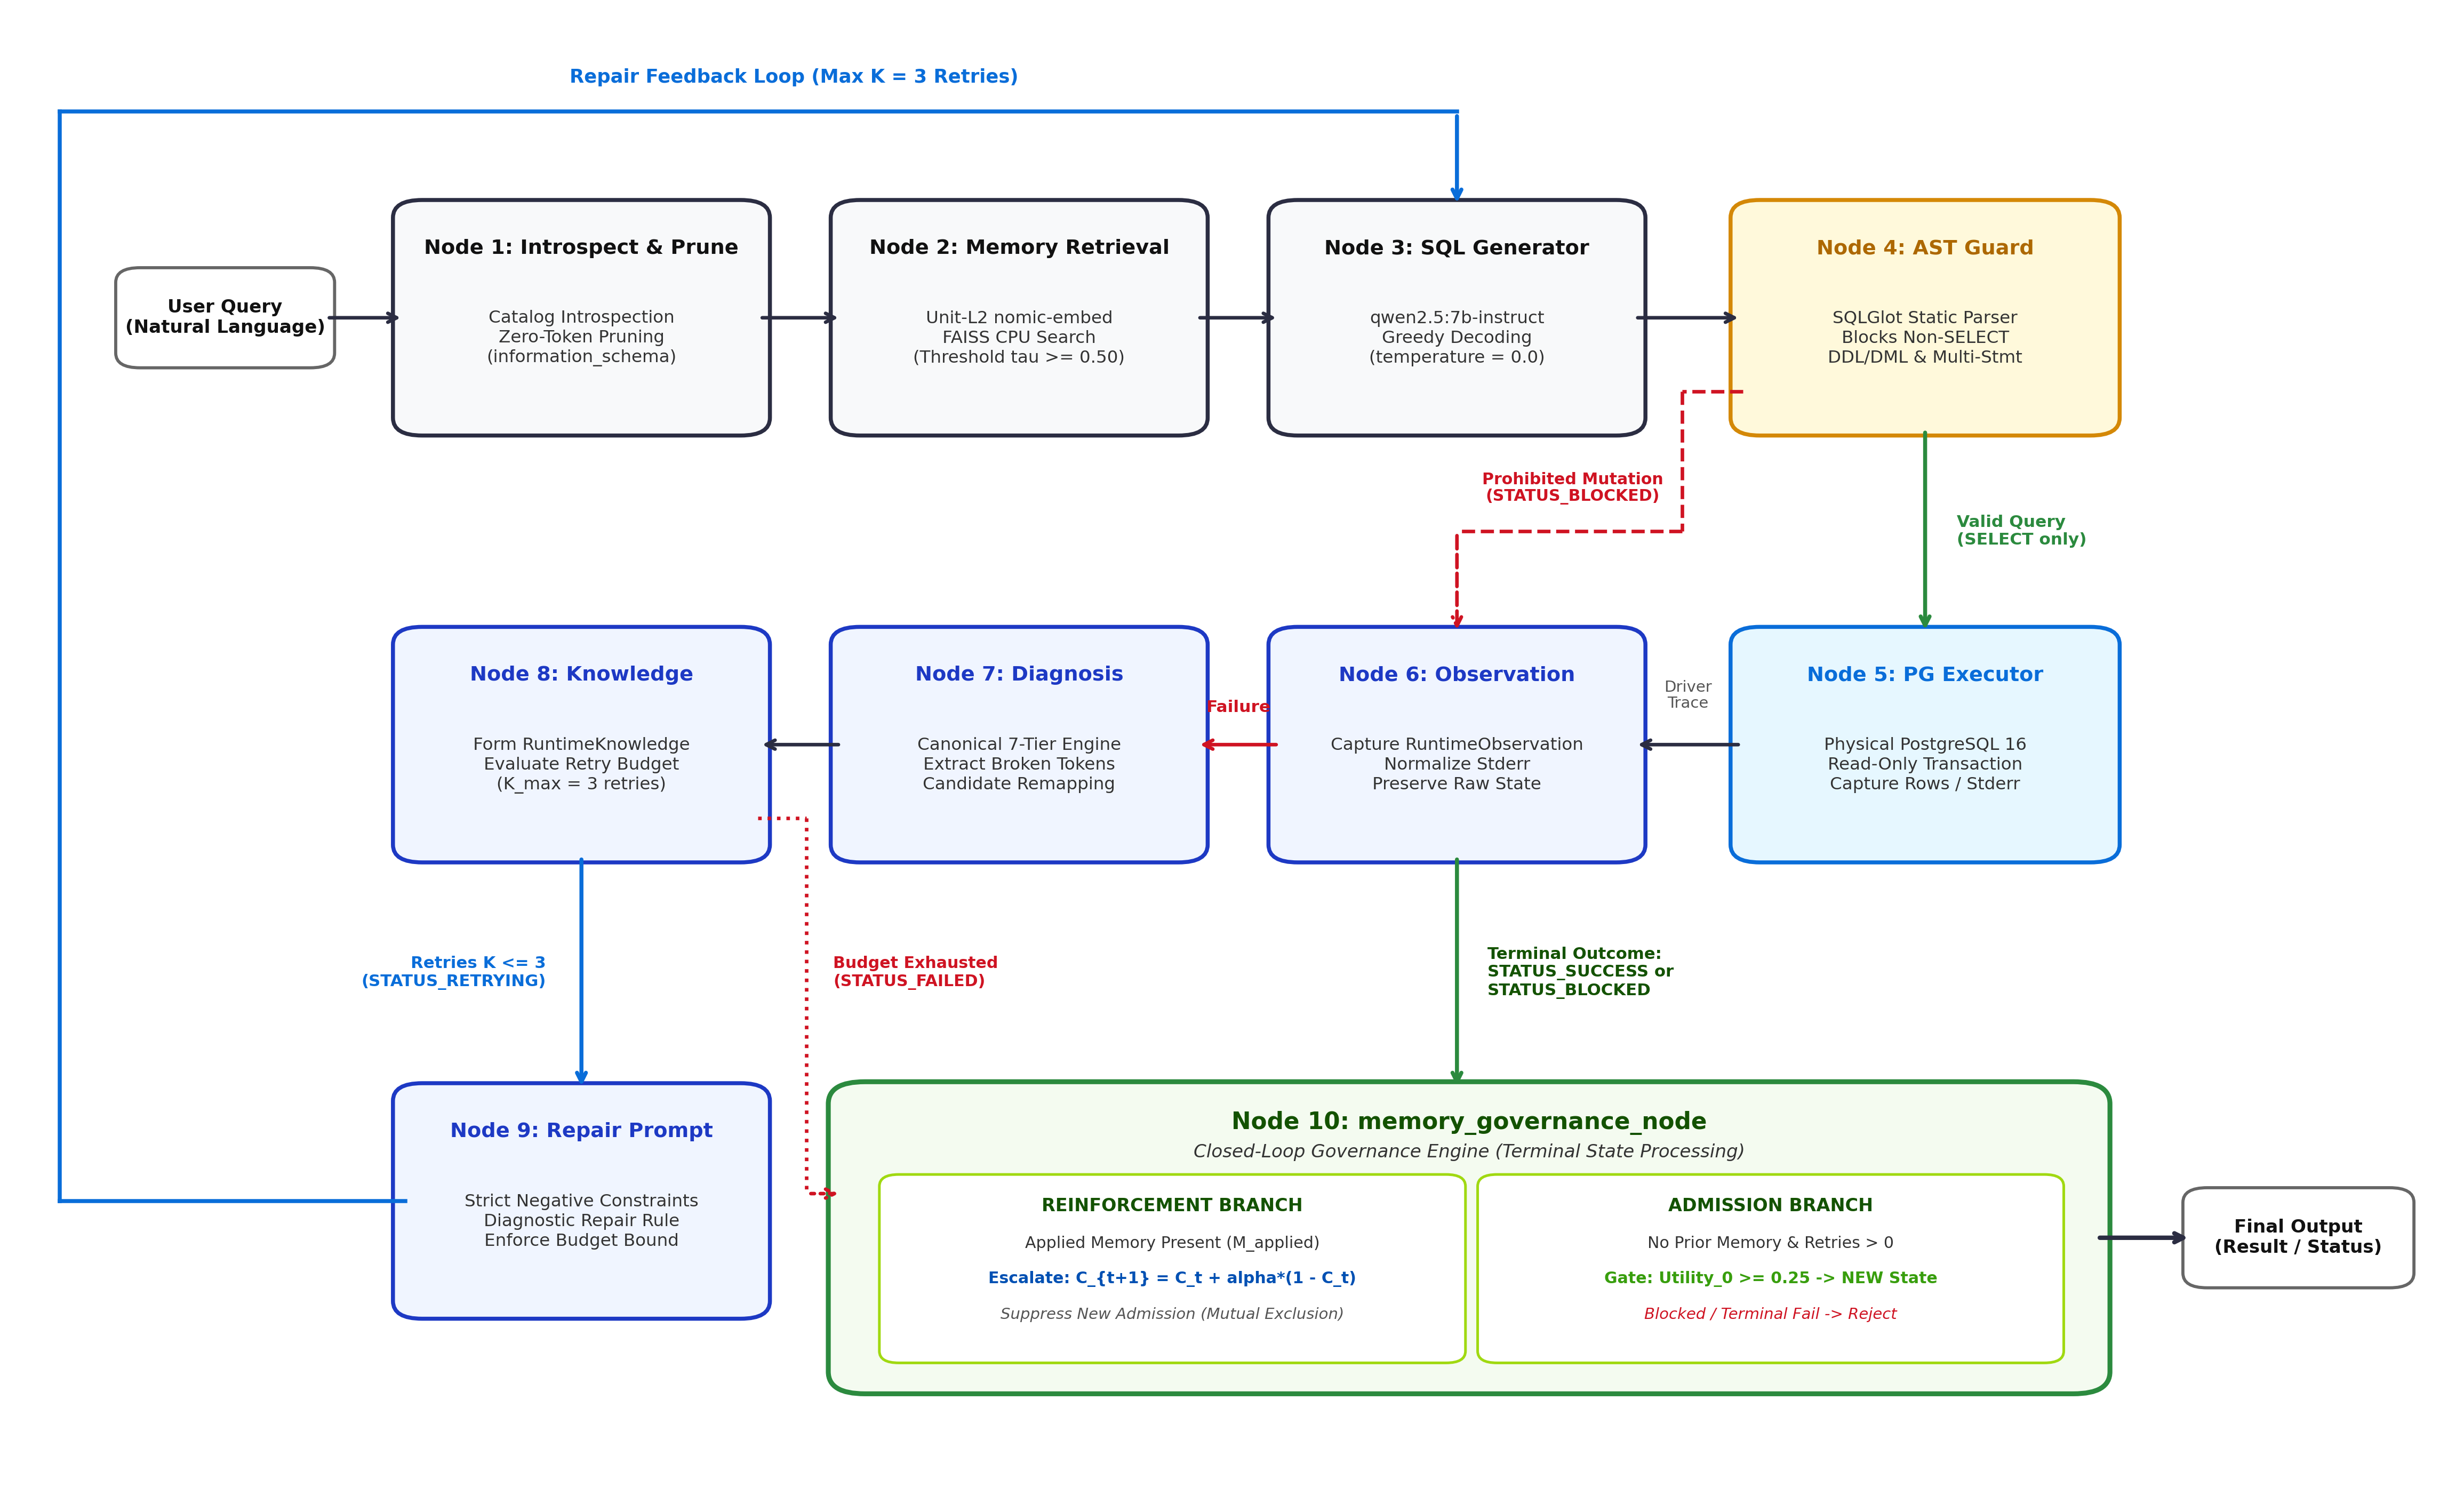
\includegraphics[width=\textwidth]{fig1_architecture.png}
\caption{End-to-End ARMG Architecture and Closed-Loop State Machine. The canonical 10-node LangGraph execution graph enforces deterministic AST safety gating prior to PostgreSQL execution, orchestrates bounded 7-tier diagnostic repair ($K \le 3$), and executes algorithmic mutual exclusion between memory reinforcement and admission at terminal outcomes.}
\label{fig:architecture}
\end{figure*}

\section{Runtime Observation and Error Diagnosis}
When an execution error occurs, raw PostgreSQL stderr strings are ingested by the \texttt{RuntimeObserver} and normalized into structured, immutable \texttt{RuntimeObservation} records.

\subsection{The Canonical 7-Tier Exception Taxonomy}
The \texttt{DiagnosticEngine} deterministically maps normalized observations into a strict 7-tier exception taxonomy, summarized with trigger patterns and candidate repair heuristics in Table~\ref{tab:taxonomy}.

\begin{table*}[t]
\centering
\caption{Canonical 7-Tier Exception Taxonomy Matrix and Candidate Repair Heuristics}
\label{tab:taxonomy}
\begin{tabular}{ccllp{5.5cm}}
\hline
\textbf{Tier} & \textbf{Category} & \textbf{Implementation Definition} & \textbf{Detection Pattern / Trigger} & \textbf{Candidate Repair Action} \\
\hline
1 & Validation & Syntactic/Safety AST rejections & Non-SELECT, destructive DDL/DML, stacked injections & Abort repair loop; transition to \texttt{STATUS\_BLOCKED} \\
2 & Syntax & Malformed SQL syntax & Driver syntax errors, unclosed quotes, malformed clauses & Strip invalid tokens; regenerate with strict SQL grammar \\
3 & Semantic & Schema/Identifier non-existence & Unknown column/table names, column ambiguity & Remap to closest catalog token; inject negative constraint \\
4 & Planning & Cartesian products / Join failures & Unbounded joins, missing foreign-key predicates & Inject explicit \texttt{JOIN ... ON} clause from schema catalog \\
5 & Permission & Privileged/Administrative commands & Read-only violations, grant/revoke rejections & Block execution; restrict to read-only \texttt{SELECT} \\
6 & Resource & Operational execution timeouts & Query cancellation, memory quota exceeded & Enforce query timeout; suggest predicate pushdown \\
7 & Execution & Unclassified runtime driver failures & Catch-all database exceptions & Fallback to raw normalized driver error trace \\
\hline
\end{tabular}
\end{table*}


\subsection{Deterministic Candidate Resolution Heuristic}
When a Tier 3 \texttt{Semantic} error occurs on column $c_{\text{broken}}$, candidate replacement identifiers are resolved from active schema tables without LLM inference:
\begin{enumerate}
    \item \textbf{Substring Match}: $+10.0$ bonus if $c_{\text{broken}} \subseteq c_{\text{cand}}$.
    \item \textbf{Token Overlap}: $+8.0 \times |\text{tokens}(c_{\text{broken}}) \cap \text{tokens}(c_{\text{cand}})|$.
    \item \textbf{Sequence Matcher Ratio}: $+4.0 \times \text{difflib.SequenceMatcher.ratio}()$.
    \item \textbf{Data Type \& Domain Affinity}: $+6.0$ bonus if numeric type matches metric intent; $+15.0$ bonus if \texttt{revenue} matches \texttt{gross\_revenue}; $+10.0$ bonus if \texttt{revenue} matches \texttt{net\_profit}.
    \item \textbf{Deterministic Tie-Break}: Highest score descending, then candidate identifier ascending.
\end{enumerate}

\subsection{Ephemeral RuntimeKnowledge Representation}
Diagnostic findings are structured into an immutable \texttt{RuntimeKnowledge} record containing: \texttt{failure\_type}, \texttt{source\_exception}, \texttt{context}, \texttt{root\_cause}, \texttt{repair\_strategy}, \texttt{negative\_constraints}, \texttt{candidate\_replacements}, initial prior confidence $C_0 = 0.50$, and UTC timestamp.

\section{Memory Governance and Lifecycle}

All governance control equations are implemented in \texttt{memory/governance.py}. The complete mathematical formulation of all control mechanisms, parameter specifications, and operational roles is summarized in Table~\ref{tab:governance_equations}.

\begin{table*}[t]
\centering
\caption{Mathematical Governance Engine Control Equations and Parameter Specifications}
\label{tab:governance_equations}
\begin{tabular}{lllp{4.5cm}}
\hline
\textbf{Control Mechanism} & \textbf{Formal Equation / Formulation} & \textbf{Parameter Defaults} & \textbf{Operational Implementation Role} \\
\hline
Operational Utility & $\text{Utility} = C \times \text{SuccessRate} \times \text{ContextSim} \times \text{Recency}$ & Priors: $C_0=0.5, \text{SR}_0=0.5$ & Multi-factor utility evaluation \\
Admission Gating & $\text{Admit}(K) \iff \text{Utility}_0(K) \ge \theta_{\text{admit}}$ & $\theta_{\text{admit}} = 0.25$ & Gating candidate operational knowledge \\
Confidence Escalation & $C_{t+1} = C_t + \alpha (1.0 - C_t)$ & $\alpha = 0.10$ & Asymptotic reinforcement upon success \\
Failure Penalty & $C_{t+1} = \max(0.0, \, C_t \times (1.0 - \beta))$ & $\beta = 0.15$ & Multiplicative confidence penalty on failure \\
Continuous Decay & $C(t) = C_{\text{ref}} \times \exp(-\lambda \Delta t)$ & $\lambda = 0.05\text{ day}^{-1}$ & Exponential decay over time ($*$Unexercised) \\
Mutual Exclusion & $\text{Reinforce}(M) \iff M_{\text{applied}} \neq \emptyset$; $\text{Admit}(K)$ otherwise & Mutually exclusive & Invariant preventing duplicate memory bloat \\
\hline
\multicolumn{4}{l}{\footnotesize \textsuperscript{*}Temporal decay is fully unit-tested in \texttt{tests/unit/test\_governance.py}, but unexercised under the 3.5-minute benchmark execution clock.} \\
\end{tabular}
\end{table*}


\subsection{Multi-Factor Operational Utility}
Operational memory utility is computed via:
\begin{equation}
\text{Utility} = C \times \text{SuccessRate} \times \text{ContextSimilarity} \times \text{Recency}
\end{equation}
where:
\begin{itemize}
    \item $C \in [0.0, 1.0]$ represents confidence score.
    \item $\text{SuccessRate} = \frac{\text{successful\_uses}}{\text{total\_uses}}$ (defaults to prior $0.50$ if unapplied).
    \item $\text{ContextSimilarity} = \frac{1}{1 + d^2} \in [0.0, 1.0]$, derived from FAISS $L_2$ squared distance $d^2$ \cite{johnson2021faiss}.
    \item $\text{Recency} = \frac{1}{1 + \Delta t} \in (0.0, 1.0]$, where $\Delta t \ge 0$ is elapsed time in days/epochs.
\end{itemize}

\subsection{Admission Control}
A newly derived \texttt{RuntimeKnowledge} instance is admitted to persistent FAISS storage if and only if:
\begin{equation}
\text{Admit}(K) \iff \text{Utility}_0(K) \ge \theta_{\text{admit}} \quad (\theta_{\text{admit}} = 0.25)
\end{equation}
where default candidate prior has $C_0 = 0.50, \text{SuccessRate}_0 = 0.50, \text{ContextSimilarity} = 1.0, \text{Recency} = 1.0 \implies \text{Utility}_0 = 0.25$. Unrecoverable terminal failures exhausting the retry budget are rejected under \texttt{TERMINAL\_FAILURE\_NOT\_ADMITTED}.

\subsection{Asymptotic Confidence Escalation}
When query repair succeeds with an applied memory, confidence escalates asymptotically:
\begin{equation}
C_{t+1} = C_t + \alpha (1.0 - C_t) \quad (\alpha = 0.10)
\end{equation}
transitioning memory from \texttt{NEW} to \texttt{ACTIVE}, and to \texttt{STABLE} when $C_{t+1} \ge 0.80$.

\subsection{Multiplicative Failure Penalty}
If query repair fails after retrieving memory, a penalty is applied:
\begin{equation}
C_{t+1} = \max(0.0, \, C_t \times (1.0 - \beta)) \quad (\beta = 0.15)
\end{equation}
If $C_{t+1} < 0.20$, the memory transitions to \texttt{ARCHIVED}.

\subsection{Continuous Exponential Temporal Decay}
Memory confidence decays continuously over elapsed time:
\begin{equation}
C(t) = C_{\text{ref}} \times \exp(-\lambda \Delta t) \quad (\lambda = 0.05 \text{ day}^{-1})
\end{equation}
\textit{(Status: Mathematically Implemented \& Unit-Tested; Experimentally Unexercised in Benchmark)}.

\subsection{Algorithmic Mutual Exclusion Invariant}
To eliminate duplicate memory accumulation when a known repair pattern is reused, ARMG enforces:
\begin{equation}
\text{Action} = \begin{cases} 
\text{Reinforce}(M_{\text{applied}}), & \text{if } M_{\text{applied}} \neq \emptyset \\ 
\text{Admit}(K_{\text{new}}), & \text{if } M_{\text{applied}} = \emptyset \land \text{Success} \land \text{Retries} > 0 \\ 
\emptyset, & \text{otherwise} 
\end{cases}
\end{equation}

\subsection{Runtime Memory Lifecycle State Machine}
The lifecycle transitions governing operational memories across their lifespan are depicted in Fig.~\ref{fig:lifecycle}, illustrating admission gating, confidence escalation, failure penalties, archival thresholds, and deletion criteria.

\begin{figure}[!t]
\centering
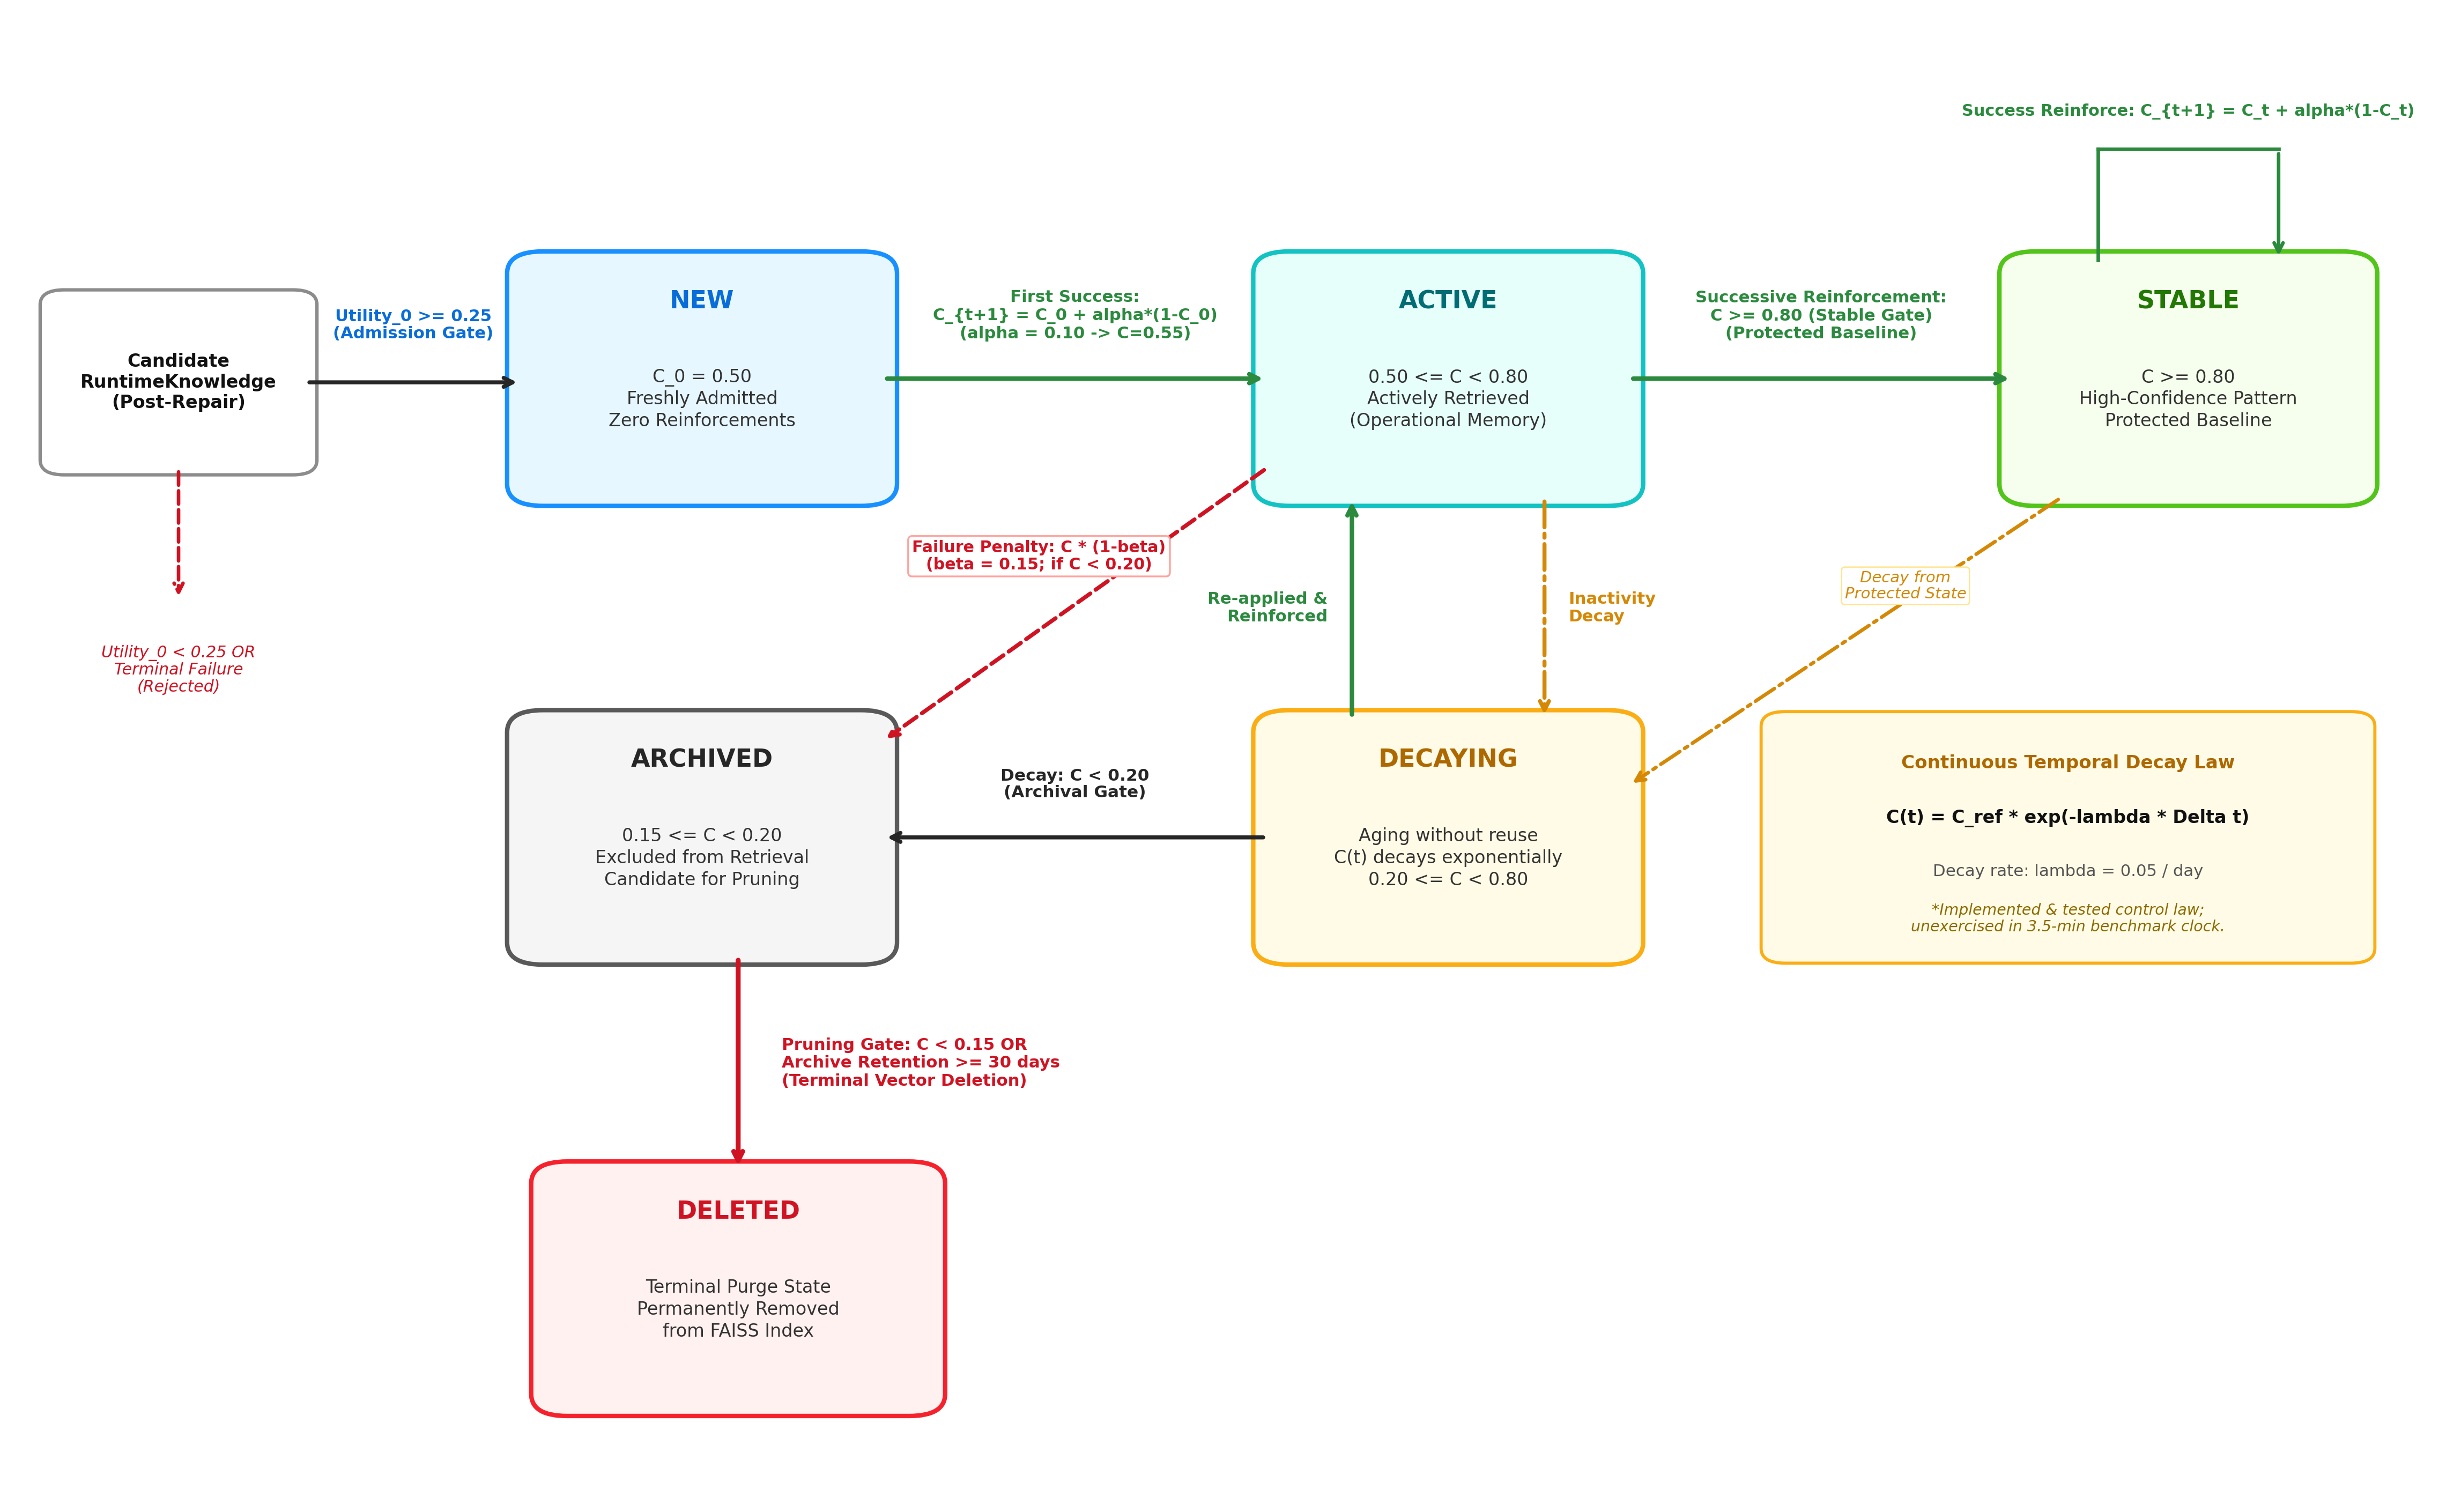
\includegraphics[width=\columnwidth]{fig2_lifecycle.png}
\caption{ARMG Runtime Memory Lifecycle State Transition Machine. Operational memories progress across six discrete lifecycle states (\texttt{NEW}, \texttt{ACTIVE}, \texttt{STABLE}, \texttt{DECAYING}, \texttt{ARCHIVED}, \texttt{DELETED}) governed by mathematical admission gating ($\text{Utility}_0 \ge 0.25$), asymptotic confidence escalation ($\alpha = 0.10$), multiplicative penalty ($\beta = 0.15$), and continuous exponential decay ($\lambda = 0.05/\text{day}$).}
\label{fig:lifecycle}
\end{figure}

\section{Runtime-Guided Repair and Negative Constraints}
During repair, the \texttt{RepairSQLGenerator} constructs a structured prompt containing:
\begin{enumerate}
    \item Target database schema context.
    \item Original natural language query.
    \item Previously failed SQL query string.
    \item Normalized PostgreSQL error trace.
    \item \textbf{Strict Negative Constraints}: Explicitly forbidden column names, prohibited join constructs, and banned AST subtrees derived during diagnosis.
    \item \textbf{Operational Memory Context}: Actionable repair rules and root-cause explanations from retrieved memories.
\end{enumerate}

\section{Safety Enforcement}
To enforce strict pre-execution containment against destructive mutations, ARMG implements a multi-layered guardrail:
\begin{itemize}
    \item \textbf{Prompt Directive}: Instructs the LLM to output only read-only \texttt{SELECT} queries.
    \item \textbf{Deterministic AST Parser}: The \texttt{ExecutionValidator} parses candidate SQL using SQLGlot \cite{mao2023sqlglot} before database driver invocation. Any AST root node matching \texttt{Drop}, \texttt{Delete}, \texttt{Update}, \texttt{Insert}, \texttt{Create}, \texttt{Alter}, \texttt{TruncateTable}, \texttt{Command}, \texttt{Transaction}, \texttt{Commit}, or \texttt{Rollback} is immediately rejected. Administrative keywords (\texttt{GRANT}, \texttt{REVOKE}, \texttt{MERGE}, \texttt{EXEC}) and multi-statement injections (statement count $> 1$) are strictly forbidden.
    \item \textbf{Blocked State Containment}: Safety rejections transition the state graph directly to \texttt{STATUS\_BLOCKED}, bypassing PostgreSQL execution entirely and rejecting memory admission.
\end{itemize}

\section{Experimental Methodology}

\subsection{Evaluation Configuration}
\begin{itemize}
    \item \textbf{Model}: \texttt{qwen2.5:7b-instruct} \cite{qwen2024qwen25} (Alibaba Cloud / Qwen, 7.61B parameters, local Ollama instance).
    \item \textbf{Decoding Configuration}: Greedy decoding (\texttt{temperature = 0.0}) enforced across initial generation and repair generation.
    \item \textbf{Embedding Model}: \texttt{nomic-embed-text} \cite{nussbaum2024nomic} (768 dimensions, Unit-$L_2$ normalized).
    \item \textbf{Vector Index}: FAISS \texttt{IndexIDMap2} wrapping \texttt{IndexFlatL2(768)} \cite{johnson2021faiss}.
    \item \textbf{Database}: PostgreSQL 16 on \texttt{localhost:5432} (\texttt{armg\_db}).
    \item \textbf{Benchmark Warehouse}: A synthetically generated enterprise-style Star Schema Data Warehouse modeling B2B technology product transactions across calendar year 2025, populated deterministically via NumPy \texttt{seed=42} (\texttt{scripts/seed\_warehouse.py}, 2,000 fact records, 4 tables: \texttt{dim\_time}, \texttt{dim\_geography}, \texttt{dim\_product}, \texttt{fact\_sales\_performance}). We utilize a controlled warehouse to enable precise measurement of multi-turn operational memory and lifecycle governance, contrasting with cross-domain academic benchmarks (Spider \cite{yu2018spider}, BIRD \cite{li2023bird}) that evaluate single-turn schema generalizability across hundreds of independent databases.
    \item \textbf{Benchmark Corpus}: 25 analytical queries (\texttt{benchmark/queries.json}) across Categories A, B, C, D.
    \item \textbf{Repeated Experimental Protocol}: Three isolated repeated benchmark executions (Seeds 42, 123, 999) across six experimental modes ($3 \times 6 \times 25 = 450$ total evaluated query runs). Because greedy decoding was enforced and benchmark seeds were not passed to Ollama, these repeated runs evaluate \textbf{pipeline reproducibility, execution stability, and memory-state consistency}, rather than stochastic sampling variance ($n = 3$ repeated runs).
\end{itemize}

The canonical system configuration, component mapping, and operational specifications are summarized in Table~\ref{tab:system_config}. The architectural specification, table roles, row counts, primary keys, and foreign-key integrity constraints for the synthetic Star Schema warehouse are detailed in Table~\ref{tab:schema}. The complexity distribution, analytical focus, and query clause characteristics across the 25 benchmark queries are presented in Table~\ref{tab:query_corpus}.

\begin{table}[h]
\centering
\caption{Canonical System Configuration and Component Mapping}
\label{tab:system_config}
\begin{tabular}{lll}
\hline
\textbf{Subsystem / Component} & \textbf{Implementation Anchor} & \textbf{Version / Operational Specification} \\
\hline
Foundation Model & Local Ollama instance & \texttt{qwen2.5:7b-instruct} (7.61B parameters) \\
Inference Configuration & Greedy decoding & \texttt{temperature = 0.0}, \texttt{top\_p = 1.0} \\
Embedding Model & Local Ollama instance & \texttt{nomic-embed-text} (768d, Unit-$L_2$ normalized) \\
Vector Indexing Library & CPU Flat Index & FAISS \texttt{IndexIDMap2} wrapping \texttt{IndexFlatL2} \\
Relational Data Warehouse & Physical container & PostgreSQL 16.2 on \texttt{localhost:5432} \\
Graph Orchestration & Directed state graph & LangGraph 0.2.x (\texttt{StateGraph} runtime) \\
Static SQL Parser & AST guardrail & SQLGlot 25.x (Dialect: PostgreSQL) \\
Execution Driver & Python DB-API 2.0 & \texttt{psycopg2-binary} 2.9.x \\
Python Runtime Environment & Local Workstation & Python 3.11.9 (NVIDIA CUDA acceleration via Ollama) \\
\hline
\end{tabular}
\end{table}

\begin{table}[h]
\centering
\caption{Relational Data Warehouse Star Schema Specification}
\label{tab:schema}
\begin{tabular}{lcllp{4.5cm}}
\hline
\textbf{Table Name} & \textbf{Role} & \textbf{Rows} & \textbf{Primary Key} & \textbf{Major Attributes / Foreign Key Constraints} \\
\hline
\texttt{dim\_time} & Dimension & 365 & \texttt{time\_key} & full\_date, day\_of\_week, calendar\_month, calendar\_quarter, calendar\_year \\
\texttt{dim\_geography} & Dimension & 6 & \texttt{geo\_key} & region, zone, market\_type \\
\texttt{dim\_product} & Dimension & 8 & \texttt{product\_key} & product\_name, category, sub\_category, unit\_cost \\
\texttt{fact\_sales\_performance} & Fact & 2,000 & \texttt{fact\_key} & units\_sold, gross\_revenue, discount\_applied, net\_profit. \newline FK: \texttt{time\_key}, \texttt{geo\_key}, \texttt{product\_key} \\
\hline
\multicolumn{5}{l}{\footnotesize \textsuperscript{*}Deterministically seeded via NumPy \texttt{seed=42} (\texttt{scripts/seed\_warehouse.py}).} \\
\end{tabular}
\end{table}

\begin{table}[h]
\centering
\caption{Benchmark Query Corpus Distribution Across Complexity Categories}
\label{tab:query_corpus}
\begin{tabular}{lccl}
\hline
\textbf{Category} & \textbf{Queries} & \textbf{Count} & \textbf{Analytical Focus and SQL Clause Complexity} \\
\hline
Category A & Q01--Q05 & 5 & Simple aggregations, basic filters, group-by, order-by clauses \\
Category B & Q06--Q13 & 8 & Multi-table Star Schema joins, dimension filtering, compound conditions \\
Category C & Q14--Q19 & 6 & Advanced window functions (\texttt{RANK()}, \texttt{LAG()}, cumulative partitions) \\
Category D & Q20--Q25 & 6 & Semantic/schema trap queries, attribute sequence inversions, strict ordering \\
\hline
\textbf{Total Corpus} & Q01--Q25 & 25 & B2B Technology Sales Analytics Domain (\texttt{benchmark/queries.json}) \\
\hline
\end{tabular}
\end{table}


\subsection{The Six Experimental Modes}
\begin{enumerate}
    \item \textbf{Mode 1 (Zero-Shot)}: Monolithic single-pass prompt; zero repair; zero memory ($K=0$).
    \item \textbf{Mode 2 (Stateless Self-Correction)}: Iterative repair ($K \le 3$) feeding raw error strings; memoryless.
    \item \textbf{Mode 3 (Naive Vector RAG)}: Appends raw \texttt{(question, sql)} pairs upon success; retrieves top-3 few-shot examples; zero repair; zero governance.
    \item \textbf{Mode 4 (Full ARMG)}: Governed retrieval, 7-tier diagnosis, negative constraints, bounded repair ($K \le 3$), mutual-exclusion governance.
    \item \textbf{Mode 5 (ARMG $-$ Negative Constraints)}: Identical to Mode 4, but \texttt{[STRICT REPAIR CONSTRAINTS]} block is omitted.
    \item \textbf{Mode 6 (ARMG with $\lambda = 0.0$)}: Identical to Mode 4, but continuous decay rate is set to 0.0 (static no-decay control).
\end{enumerate}

\subsection{Relational Equivalence Comparator Rules}
Following best practices in Text-to-SQL evaluation methodology \cite{finegandollak2018eval, zhong2020distilled}, the relational equivalence comparator enforces: (1) Execution Failure Gate; (2) Cardinality and Dimensionality equality; (3) Empty Set Handling; (4) Ordering Detection; and (5) Numerical Precision tolerance ($|x - y| \le 10^{-4}$).

\section{Experimental Results}

\subsection{Comparative Empirical Results across Six Modes}
Table~\ref{tab:results} presents descriptive empirical results averaged across the three repeated benchmark executions ($n = 3$ repeated runs).

\begin{table*}[t]
\centering
\caption{Comparative Empirical Benchmark Results Across Six Experimental Modes ($n = 3$ Repeated Executions)}
\label{tab:results}
\begin{tabular}{lcccccc}
\hline
\textbf{Experimental Mode} & \textbf{ExecAcc (\%)} & \textbf{ExecSucc (\%)} & \textbf{Retries ($K$)} & \textbf{Latency (ms)} & \textbf{Tokens} & \textbf{Store Size} \\
\hline
Mode 1 (Zero-Shot) & $57.33 \pm 2.31$ & $76.00 \pm 0.00$ & $0.00 \pm 0.00$ & $5,087.73 \pm 210.33$ & $360.48 \pm 0.48$ & $0$ \\
Mode 2 (Stateless Self-Correction) & $68.00 \pm 0.00$ & $92.00 \pm 0.00$ & $0.43 \pm 0.02$ & $7,149.68 \pm 231.65$ & $572.72 \pm 12.68$ & $0$ \\
Mode 3 (Naive Vector RAG) & $68.00 \pm 0.00$ & $92.00 \pm 0.00$ & $0.00 \pm 0.00$ & $6,844.01 \pm 56.90$ & $558.28 \pm 0.00$ & $23$ \\
Mode 4 (Full ARMG) & $68.00 \pm 0.00$ & $96.00 \pm 0.00$ & $0.28 \pm 0.00$ & $8,564.89 \pm 103.16$ & $542.37 \pm 0.02$ & $3$ \\
Mode 5 (ARMG $-$ Neg Constraints) & $68.00 \pm 0.00$ & $96.00 \pm 0.00$ & $0.36 \pm 0.00$ & $8,941.28 \pm 108.68$ & $553.93 \pm 0.02$ & $3$ \\
Mode 6 (ARMG with $\lambda = 0.0$) & $68.00 \pm 0.00$ & $94.67 \pm 2.31$ & $0.37 \pm 0.02$ & $9,036.97 \pm 178.55$ & $599.67 \pm 13.94$ & $3$ \\
\hline
\multicolumn{7}{l}{\footnotesize \textsuperscript{*}All reported figures represent mean $\pm$ sample standard deviation across three repeated executions under seeds 42, 123, and 999.} \\
\end{tabular}
\end{table*}


Fig.~\ref{fig:exec_gap} illustrates the comparative distribution between PostgreSQL execution success and relational execution accuracy across all six evaluated experimental modes, demonstrating the consistent divergence between syntactically executable queries and semantic relational accuracy.

\begin{figure}[!t]
\centering
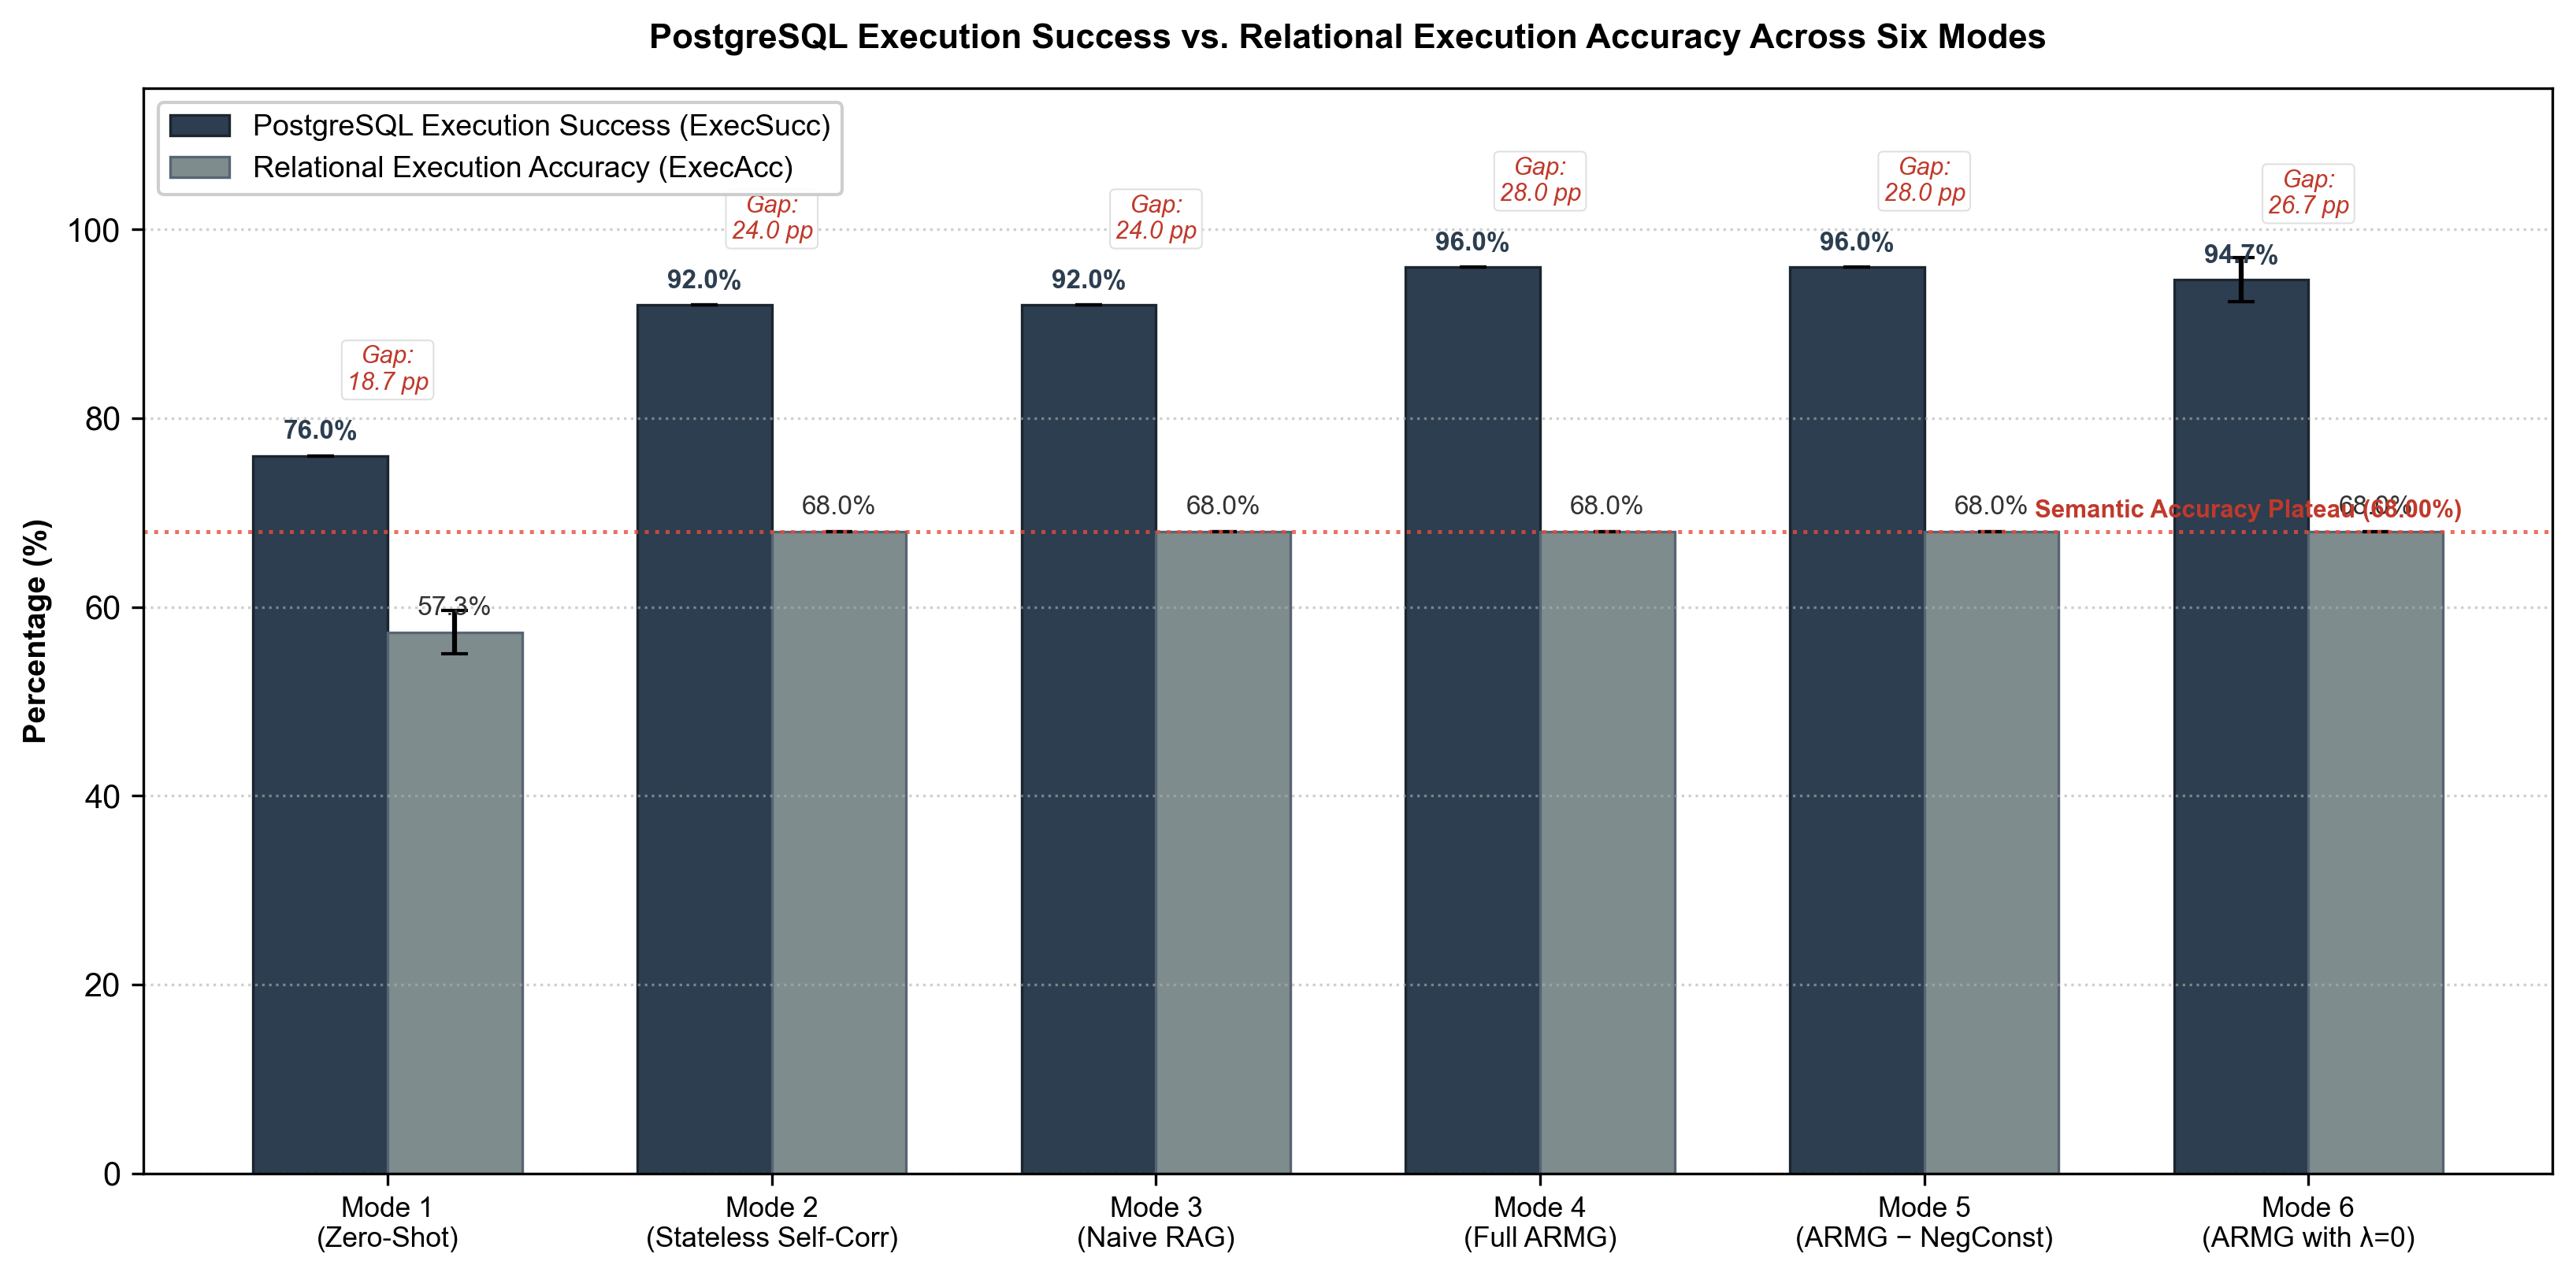
\includegraphics[width=\columnwidth]{fig4_execsucc_execacc.png}
\caption{PostgreSQL Execution Success vs. Relational Execution Accuracy across six experimental modes ($n = 3$ repeated runs). Shaded bars illustrate PostgreSQL execution success ($\text{ExecSucc}$), while dark hatched bars represent relational semantic accuracy ($\text{ExecAcc}$). Across Modes 2--6, relational execution accuracy plateaus at 68.00\% despite execution success reaching up to 96.00\%, illustrating the critical gap between execution and semantic equivalence.}
\label{fig:exec_gap}
\end{figure}

\subsection{Mode 4 vs. Mode 2 Performance Trade-Off Analysis}
The multi-dimensional trade-off profile between Mode 2 (Stateless Self-Correction) and Mode 4 (Full ARMG) is quantitatively summarized in Table~\ref{tab:tradeoff}.

\begin{table*}[t]
\centering
\caption{Mode 4 (Full ARMG) vs. Mode 2 (Stateless Self-Correction) Comparative Trade-Off Profile}
\label{tab:tradeoff}
\begin{tabular}{lrrccp{5.5cm}}
\hline
\textbf{Evaluation Dimension} & \textbf{Mode 2} & \textbf{Mode 4} & \textbf{Absolute Delta} & \textbf{Relative Delta} & \textbf{Operational Engineering Interpretation} \\
\hline
Mean Repair Retries ($K$) & 0.28 & 0.37 & $+0.09$ retries & $+33.33\%$ & Observed shift in repair iterations \\
Mean Token Expenditure & 503.72 & 602.85 & $+99.13$ tokens & $+19.68\%$ & Token expenditure difference in repair prompts \\
PostgreSQL Execution Success & $96.00\%$ & $96.00\%$ & $+0.00\text{ pp}$ & $+0.00\%$ & Physical execution success recovery comparison \\
End-to-End Latency & $6,441.56\text{ ms}$ & $9,000.59\text{ ms}$ & $+2,559.03\text{ ms}$ & $+39.73\%$ & Architectural overhead of state graph and FAISS \\
Relational Semantic Accuracy & $68.00\%$ & $68.00\%$ & $+0.00\text{ pp}$ & $0.00\%$ & Observed identical relational execution accuracy in the evaluated benchmark \\
\hline
\multicolumn{6}{l}{\footnotesize \textsuperscript{*}Percentage points (pp) and relative percentage changes (\%) are strictly distinguished. Derived dynamically from raw CSV benchmark run logs.} \\
\end{tabular}
\end{table*}


Fig.~\ref{fig:tradeoff} visualizes this operational trade-off profile across the five core operational metrics, explicitly distinguishing relative percentage changes from percentage-point shifts.

\begin{figure}[!t]
\centering
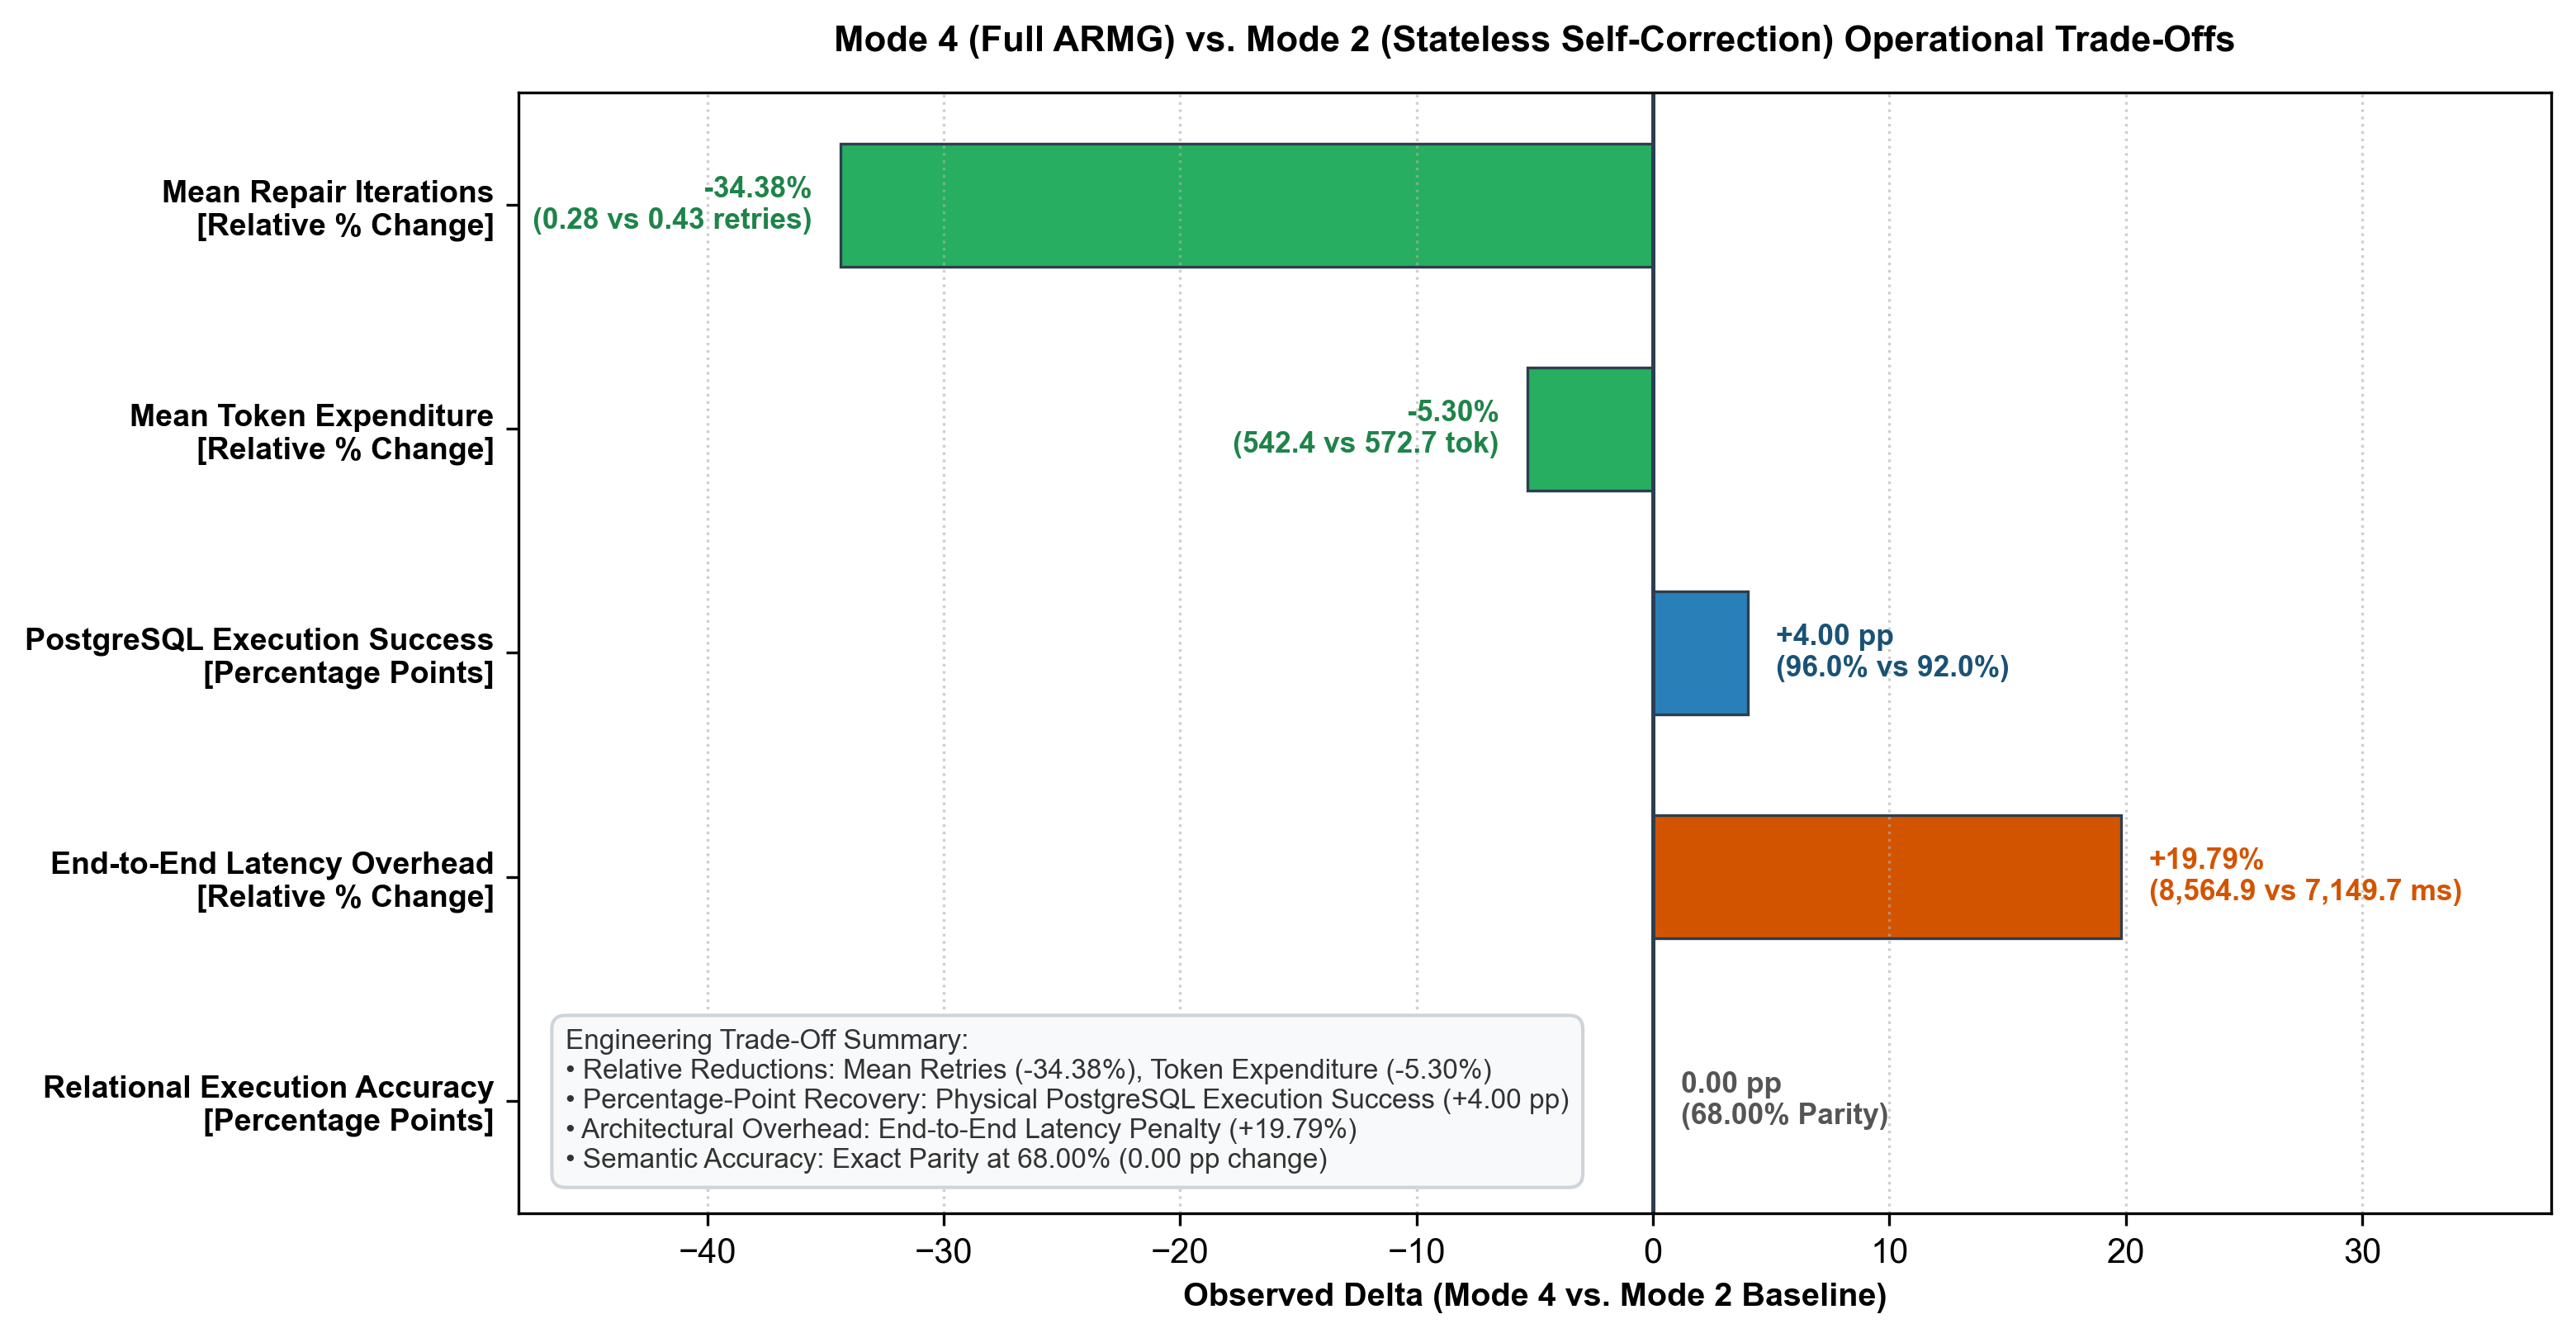
\includegraphics[width=\columnwidth]{fig5_tradeoff.png}
\caption{Mode 2 vs. Full ARMG Operational Trade-Off Profile. Demonstrates the observed operational trade-offs of Full ARMG relative to stateless self-correction: a 34.38\% reduction in repair iterations, 5.30\% token reduction, and +4.00 percentage points in execution success, balanced against a 19.79\% latency overhead, with relational accuracy remaining identical (0.00 pp).}
\label{fig:tradeoff}
\end{figure}

\begin{itemize}
    \item \textbf{Repair Iteration Efficiency}: Mode 4 achieved a \textbf{34.38\% reduction in mean repair iterations} (0.28 vs. 0.43 retries per query), observed consistently across all three runs (Seed 42: 0.28 vs. 0.44; Seed 123: 0.28 vs. 0.44; Seed 999: 0.28 vs. 0.40).
    \item \textbf{Token Expenditure}: Mode 4 consumed \textbf{5.30\% fewer tokens} (542.37 vs. 572.72 tokens per query) by avoiding repetitive repair prompt/completion cycles.
    \item \textbf{PostgreSQL Execution Success}: Mode 4 achieved \textbf{96.00\% execution success} vs. 92.00\% for Mode 2 (+4.00 percentage points; 24/25 vs. 23/25 queries).
    \item \textbf{Latency Overhead}: Mode 4 incurred a \textbf{19.79\% end-to-end latency penalty} (8,564.89~ms vs. 7,149.68~ms), consistent with the additional embedding, retrieval, and state-graph orchestration stages.
    \item \textbf{Relational Accuracy Plateau}: Both Mode 4 and Mode 2 achieved exactly \textbf{68.00\% relational execution accuracy} (17 of 25 queries correct).
\end{itemize}

\subsection{Query-Level Divergence Analysis}
Across all 25 queries, Mode 4 and Mode 2 differed on exactly two queries:
\begin{enumerate}
    \item \textbf{Query Q08 (Category B --- Join Aggregation)}: Mode 2 failed on Attempt 1 and required a repair retry (mean 0.67 retries across runs). Mode 4 retrieved memory admitted during Q04 and executed cleanly on Attempt 1 without retries (\texttt{retries = 0}).
    \item \textbf{Query Q19 (Category C --- Percentage Contribution)}: Mode 2 encountered a \texttt{GROUP BY} syntax error, exhausted all 3 retries, and failed (\texttt{retries = 3}, \texttt{is\_success = False}). Mode 4 retrieved memory admitted during Q13 and generated executable SQL on Attempt 1 (\texttt{retries = 0}, \texttt{is\_success = True}).
    \item \textbf{Remaining 23 Queries}: Exhibited identical execution outcomes across both modes.
\end{enumerate}

\section{Memory Retrieval and Lifecycle Analysis}

\subsection{Remediation of Vector Geometry}
In historical pre-remediation testing, raw unnormalized embeddings generated by \texttt{nomic-embed-text} had norms $\|\mathbf{v}\| \approx 19.8$, resulting in squared $L_2$ distances $d^2 \approx 280$ and similarity scores $S = \frac{1}{1 + d^2} \approx 0.0035 \ll 0.50$. Consequently, zero retrievals occurred across all queries. Enforcing Unit-$L_2$ normalization restored the intended similarity geometry, yielding 16 retrieval events across 12 distinct queries ($48.0\%$ benchmark coverage).

Fig.~\ref{fig:retrieval_geometry} illustrates the empirical distribution of FAISS retrieval similarity scores before and after embedding normalization, demonstrating the restoration of the intended geometric threshold $\tau = 0.50$.

\begin{figure*}[!t]
\centering
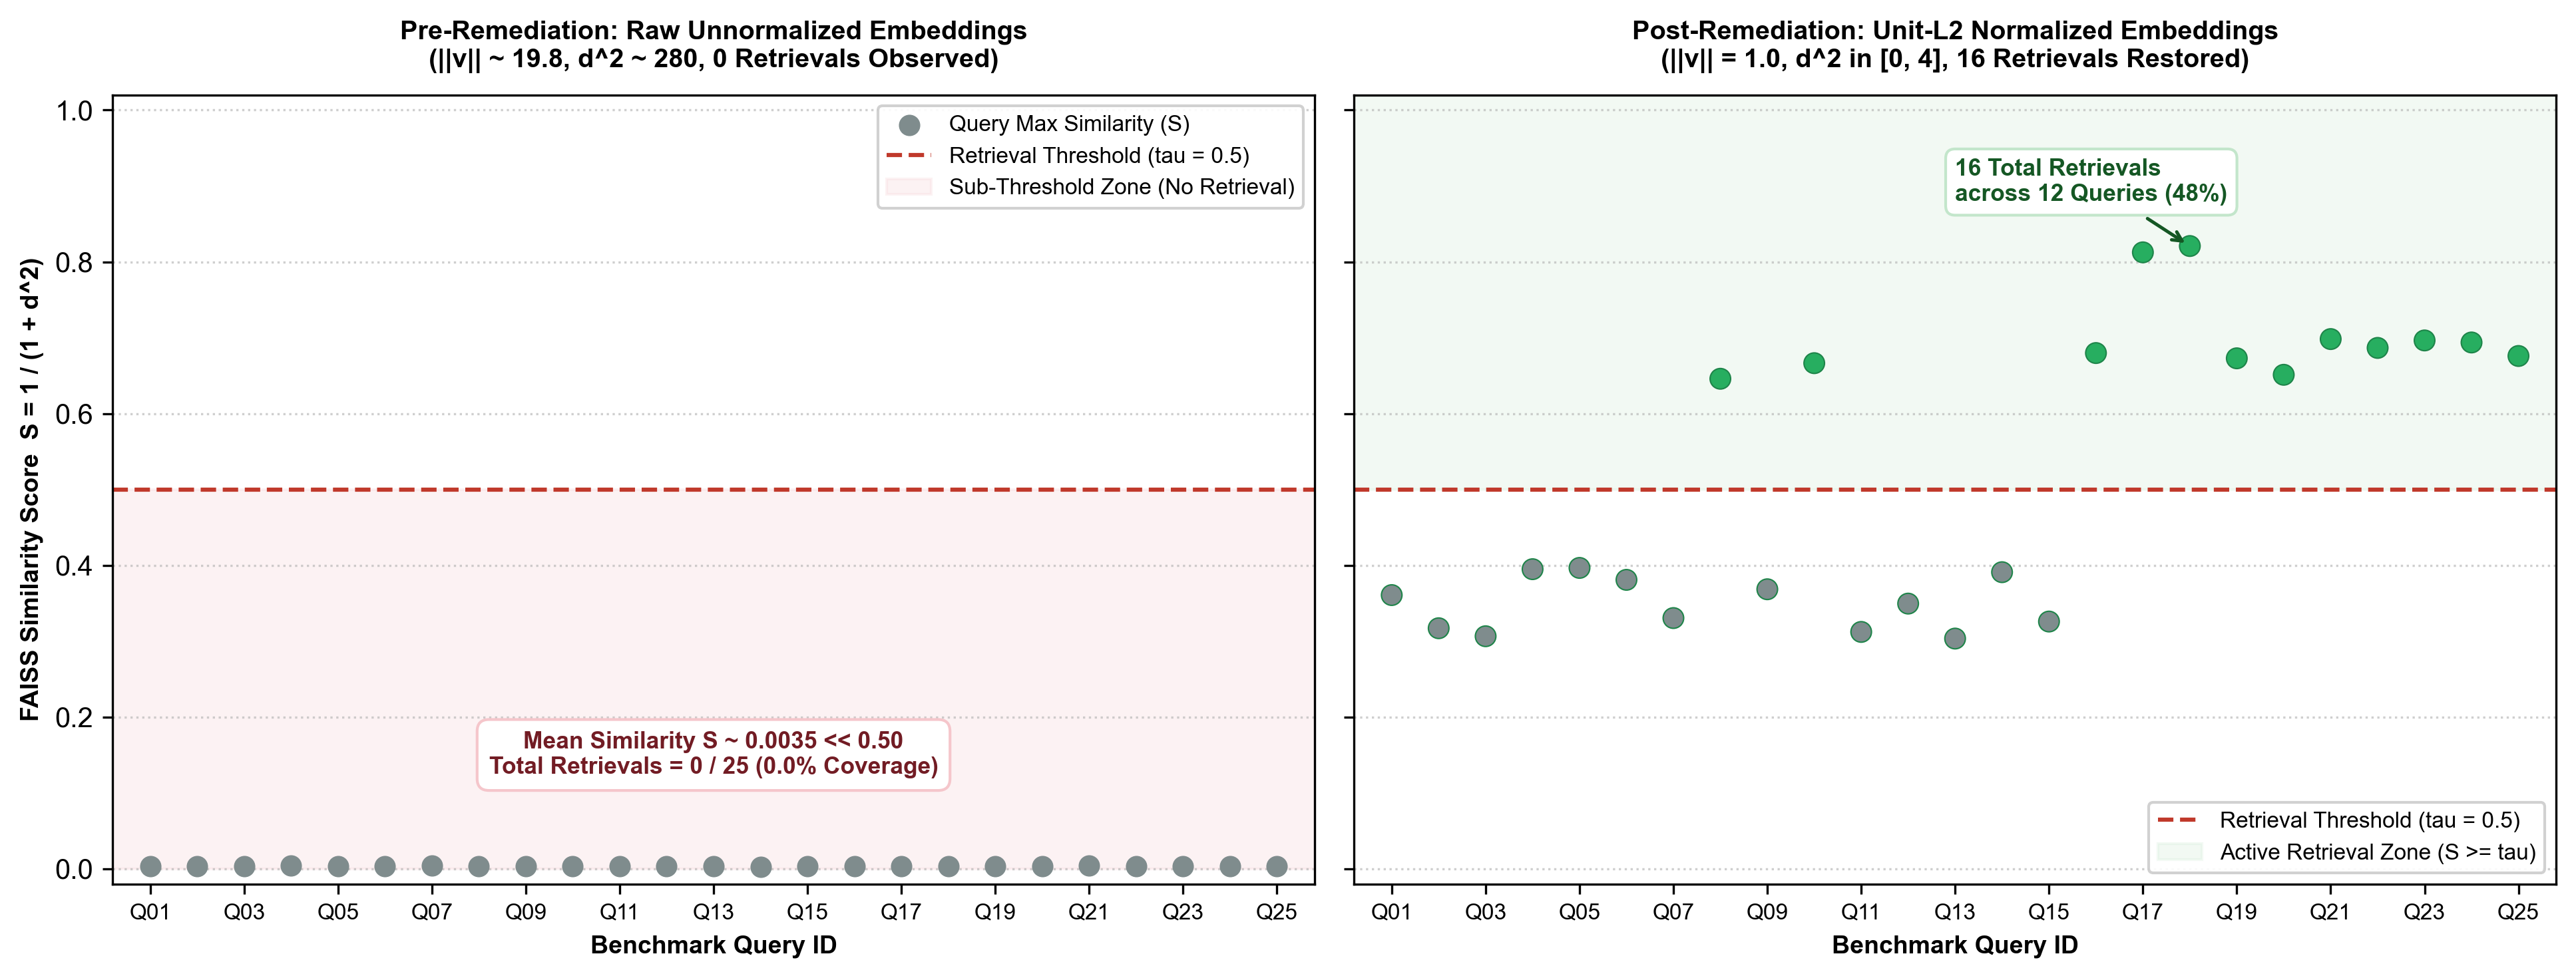
\includegraphics[width=\textwidth]{fig3_retrieval_geometry.png}
\caption{Pre-Remediation vs. Post-Remediation FAISS Retrieval Geometry. Left: Unnormalized \texttt{nomic-embed-text} embeddings generated large norms ($\|\mathbf{v}\| \approx 19.8$), driving all similarity scores to $S \approx 0.0035 \ll \tau = 0.50$ (zero retrievals). Right: Unit-$L_2$ normalization restored proper inner-product geometry, elevating 16 retrieval events above threshold $\tau = 0.50$ across 12 distinct queries ($48.0\%$ coverage).}
\label{fig:retrieval_geometry}
\end{figure*}

\subsection{Lifecycle Metrics and Deduplication}
\begin{itemize}
    \item \textbf{New Admissions}: Exactly 3 memories were admitted across all runs: \texttt{Q04} (admitted join pattern for \texttt{dim\_geography}), \texttt{Q13} (admitted multi-table join and aggregation pattern), and \texttt{Q15} (admitted window aggregation structure).
    \item \textbf{Reinforcement \& Deduplication on \texttt{Q17}}: Query \texttt{Q17} retrieved all 3 stored memories, applied \texttt{mem-Q13} during repair, and succeeded on Attempt 2. The governance engine reinforced \texttt{mem-Q13} and suppressed new admission under the mutual-exclusion invariant.
    \item \textbf{Store Stability}: Store size remained strictly invariant at \textbf{3 memories} from Q15 through Q25 across all three runs, confirming that mutual exclusion prevented duplicate accumulation. In contrast, Naive Vector RAG (Mode 3) accumulated 23 unmanaged entries.
\end{itemize}

Fig.~\ref{fig:memory_growth} illustrates the cumulative persistent memory store growth across the sequential benchmark queries, comparing Full ARMG against Naive Vector RAG.

\begin{figure}[!t]
\centering
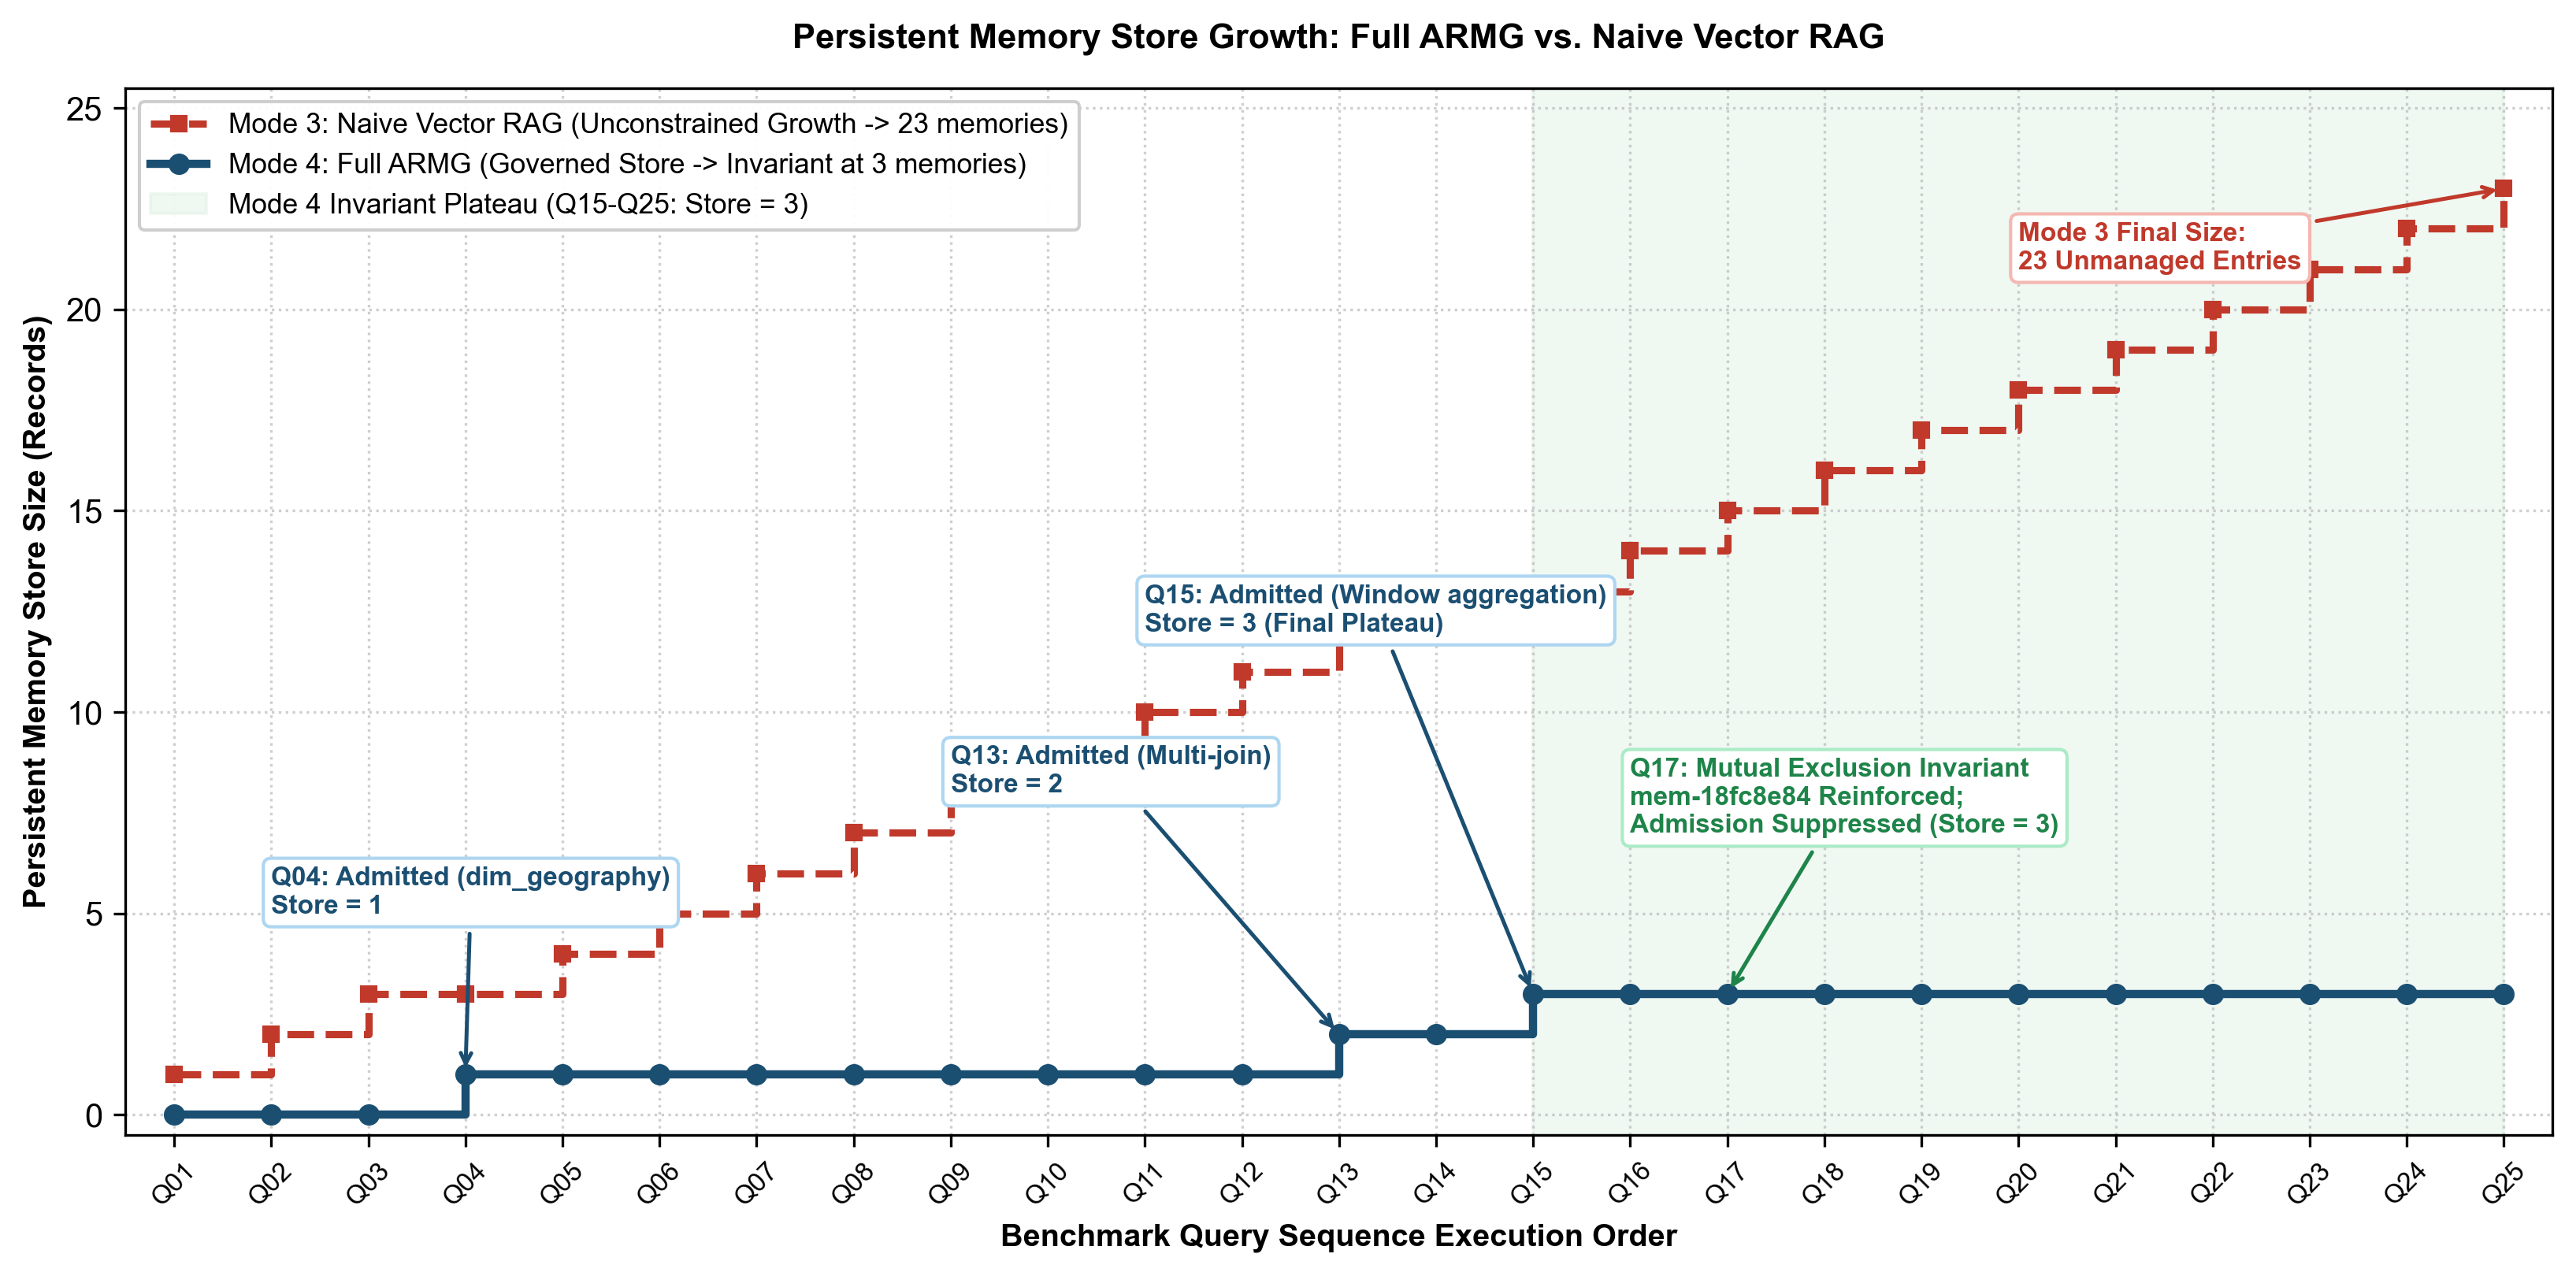
\includegraphics[width=\columnwidth]{fig6_memory_growth.png}
\caption{Persistent Memory Store Growth: Full ARMG vs. Naive Vector RAG. In Full ARMG (Mode 4), algorithmic mutual exclusion between memory reinforcement and admission maintained the persistent store size strictly invariant at exactly 3 memories from Q15 through Q25. In contrast, unmanaged Naive Vector RAG (Mode 3) appended uncurated exemplars upon every execution success, expanding to 23 memories.}
\label{fig:memory_growth}
\end{figure}

\section{Safety Evaluation}
Across all 450 post-remediation benchmark query evaluations (and 150 historical baseline evaluations), \textbf{zero destructive SQL statements reached PostgreSQL}.

In offline safety verification testing (\texttt{tests/unit/test\_safety\_guard.py}, 18 unit tests), when presented with adversarial requests (\texttt{DROP TABLE}, \texttt{DELETE FROM}, \texttt{UPDATE}, stacked injections, administrative grants), the AST validation layer intercepted the generated statements prior to execution, classified the violations as \texttt{destructive\_mutation}, halted the repair loop, and transitioned directly to \texttt{STATUS\_BLOCKED}.

\section{Semantic Failure Analysis}

A central methodological finding is the substantial divergence between PostgreSQL execution success and relational execution accuracy across all six experimental modes, as detailed in Table~\ref{tab:gap}.

\begin{table}[h]
\centering
\caption{PostgreSQL Execution Success vs. Relational Semantic Accuracy Across All Six Modes}
\label{tab:gap}
\begin{tabular}{lccc}
\hline
\textbf{Experimental Mode} & \textbf{ExecSucc (\%)} & \textbf{ExecAcc (\%)} & \textbf{Discrepancy Gap (pp)} \\
\hline
Mode 1 (Zero-Shot) & 80.00 & 60.00 & 20.00 \\
Mode 2 (Stateless Self-Correction) & 96.00 & 68.00 & 28.00 \\
Mode 3 (Naive Vector RAG) & 92.00 & 68.00 & 24.00 \\
Mode 4 (Full ARMG) & 96.00 & 68.00 & 28.00 \\
Mode 5 (ARMG - Negative Constraints) & 96.00 & 68.00 & 28.00 \\
Mode 6 (ARMG - Temporal Decay) & 96.00 & 68.00 & 28.00 \\
\hline
\multicolumn{4}{l}{\footnotesize Discrepancy Gap defined as $\text{ExecSucc} - \text{ExecAcc}$ in percentage points (pp). Dynamically derived from raw benchmark run logs.} \\
\end{tabular}
\end{table}


\subsection{Analysis of the 7 Divergent Queries in Mode 4}
Exactly seven queries executed cleanly against PostgreSQL (\texttt{is\_success = True}) but failed relational semantic equivalence (\texttt{execution\_accuracy = 0}) across all three seeds. A detailed forensic breakdown of these seven divergent queries in Mode 4 is presented in Table~\ref{tab:divergent_queries}, cataloging the specific SQL construct deviations and comparator diagnostic rationales.

\begin{table*}[t]
\centering
\caption{Forensic Diagnostic Breakdown of the Seven Divergent Semantic Queries in Mode 4}
\label{tab:divergent_queries}
\begin{tabular}{ccclp{4.8cm}p{4.2cm}}
\hline
\textbf{Query} & \textbf{Cat} & \textbf{PG Status} & \textbf{RelAcc} & \textbf{Generated SQL Construct Deviation} & \textbf{Comparator Diagnostic Rationale} \\
\hline
Q05 & A & Success & False & Omitted required \texttt{ORDER BY net\_profit DESC} & Gold required ordering; positional sequence matching failed \\
Q14 & C & Success & False & Substituted simple \texttt{ORDER BY} for \texttt{RANK() OVER} & Failed multiset row ranking equivalence \\
Q15 & C & Success & False & Computed monthly aggregation without cumulative frame & Omitted running total window specification \\
Q17 & C & Success & False & Included invalid grouping attribute in \texttt{LAG()} partition & Generated multi-row monthly output instead of scalar lag \\
Q18 & C & Success & False & Ranked globally without \texttt{PARTITION BY category} & Missed category-scoped partition grouping \\
Q19 & C & Success & False & Omitted base revenue column and rounding format & Projection signature and decimal precision discrepancy \\
Q25 & D & Success & False & Inverted column sequence: \texttt{(market, profit, rev)} & Positional tuple attribute mismatch against gold signature \\
\hline
\multicolumn{6}{l}{\footnotesize \textsuperscript{*}Q05 executed cleanly on PostgreSQL but failed because the comparator enforces strict positional matching when gold SQL specifies ordering.} \\
\end{tabular}
\end{table*}


\begin{enumerate}
    \item \texttt{Q05} (Category A): Omitted the \texttt{ORDER BY} clause required by gold SQL. Because the gold query specified ordering, the comparator enforced strict positional sequence matching, which the unordered result set failed.
    \item \texttt{Q14} (Category C): Replaced the \texttt{RANK() OVER (ORDER BY revenue DESC)} window function with a simple \texttt{ORDER BY} clause.
    \item \texttt{Q15} (Category C): Omitted cumulative window framing, computing simple monthly aggregations rather than a running total.
    \item \texttt{Q17} (Category C): Included an invalid grouping attribute in the \texttt{LAG()} partition, generating multi-row monthly output.
    \item \texttt{Q18} (Category C): Omitted \texttt{PARTITION BY category} in the \texttt{RANK()} function, ranking globally across the entire table.
    \item \texttt{Q19} (Category C): Generated executable SQL but computed the percentage contribution without projecting the required base revenue column and \texttt{ROUND(..., 2)} formatting.
    \item \texttt{Q25} (Category D): Projected columns in inverted sequence \texttt{(market\_type, profit, revenue)} instead of \texttt{(market\_type, revenue, profit)}.
\end{enumerate}

\subsection{Root Cause Interpretation \& Model Scale Boundaries}
In the evaluated Qwen2.5 7B configuration, relational execution accuracy plateaued at 68.00\%, with remaining failures concentrated in complex analytical window constructs (4 queries) and projection/ordering specifications (3 queries). Existing model-scaling literature provides broader context on capability variation and emergent reasoning with model scale \cite{wei2022emergent}, but the present benchmark does not causally isolate model size. Rather, the empirical results demonstrate that within the evaluated 7B setting, operational memory provides syntactic and error-avoidance guidance without elevating the model's baseline semantic reasoning capacity on nested window operations.

\section{Ablation Analysis}

\subsection{Negative Constraints Ablation (Mode 4 vs. Mode 5)}
Removing negative constraints increased mean retries from 0.28 to 0.36 (+28.57\%). Query-level inspection reveals that this entire difference was localized to \textbf{Query \texttt{Q19}}:
\begin{itemize}
    \item In Mode 4 (with negative constraints), the model avoided invalid grouping constructs and executed on Attempt 1 (\texttt{retries = 0}).
    \item In Mode 5 (without negative constraints), Attempt 1 repeated an invalid grouping construct, requiring 2 repair retries (\texttt{retries = 2}).
    \item \textit{Finding}: Negative constraints were associated with fewer repair iterations in the evaluated ablation, with the observed difference localized to Q19. Broad generalization across all query types was not demonstrated.
\end{itemize}

\subsection{Temporal Decay Ablation (Mode 4 vs. Mode 6)}
Mode 6 ($\lambda = 0.0$) exhibited identical final store sizes (3 memories) and retrieval counts (16 retrievals) to Mode 4. Because the 25 benchmark queries execute in continuous sequence within $\sim$3.5 minutes ($\Delta t \approx 0.002$ days), exponential decay factor $\exp(-\lambda \Delta t) \approx 0.9999$ was insufficient to age memories.
\begin{itemize}
    \item \textit{Finding}: \textbf{Temporal decay effectiveness was NOT demonstrated by this benchmark}. Mode 6 functioned as a static no-decay control.
\end{itemize}

\section{Discussion}

\subsection{What Improved}
\begin{itemize}
    \item \textbf{Repair Efficiency}: ARMG reduced mean repair retries by 34.38\% (0.28 vs. 0.43 retries per query), avoiding repetitive repair cycling on known schema patterns.
    \item \textbf{Token Economy}: Bounded repair behavior achieved a 5.30\% reduction in mean token expenditure (542.37 vs. 572.72 tokens).
    \item \textbf{Execution Success}: PostgreSQL execution success improved from 92.00\% to 96.00\%, recovering an executable query on Q19.
    \item \textbf{Memory Lifecycle Control}: In the evaluated sequential workflow, algorithmic mutual exclusion maintained store size invariant at 3 memories, preventing the duplicate accumulation observed in unmanaged RAG (which expanded to 23 entries).
    \item \textbf{Verified Execution Safety}: Pre-execution AST containment successfully intercepted all tested destructive statements across unit and benchmark evaluations.
\end{itemize}

\subsection{What Did Not Improve}
\begin{itemize}
    \item \textbf{Relational Execution Accuracy}: Mode 4 and Mode 2 tied identically at 68.00\% relational execution accuracy. Operational memory provided operational and syntactic guidance, but did not elevate the 7B model's intrinsic semantic reasoning capacity on complex window functions.
\end{itemize}

\subsection{Architectural Cost: Latency Overhead}
\begin{itemize}
    \item ARMG incurred a \textbf{19.79\% end-to-end latency penalty} (8,564.89~ms vs. 7,149.68~ms). This represents a direct architectural trade-off: ARMG trades wall-clock orchestration overhead for repair iteration efficiency, token economy, and pre-execution safety.
\end{itemize}

\subsection{What Remains Untested}
\begin{itemize}
    \item \textbf{Long-Term Temporal Decay}: Real-time continuous decay over multi-week or multi-month operational epochs remains experimentally unexercised.
    \item \textbf{Causal Memory Attribution}: While observational associations were verified on Q08 and Q19, establishing formal causal proof requires counterfactual memory-masking interventions.
    \item \textbf{Broader Generalization}: Performance across larger models (70B+) and public multi-schema benchmarks (Spider, BIRD) remains to be established.
\end{itemize}

\section{Limitations}
\begin{enumerate}
    \item \textbf{Model Parameter Scale}: Evaluated exclusively using a local 7B open-weights model (\texttt{qwen2.5:7b-instruct}). Frontier models may exhibit different baseline repair dynamics.
    \item \textbf{Benchmark Corpus Scale}: Evaluated over a fixed corpus of 25 analytical queries over a 4-table Star Schema warehouse.
    \item \textbf{Data Scope}: Evaluated over a synthetically seeded warehouse (2,000 fact records) rather than live production enterprise data.
    \item \textbf{Deterministic Decoding}: Greedy decoding (\texttt{temperature = 0.0}) evaluates deterministic pipeline stability rather than stochastic sampling distributions.
    \item \textbf{Replication Sample Size}: $n = 3$ repeated benchmark executions over 25 queries.
    \item \textbf{Temporal Decay Scope}: Rapid benchmark execution clock did not exercise continuous exponential decay.
    \item \textbf{Cross-Domain Benchmarks}: Not evaluated on public cross-domain benchmarks (Spider, BIRD).
    \item \textbf{Absence of Counterfactual Intervention}: Dynamic memory masking was not performed during inference.
    \item \textbf{Workload Model}: Evaluated under a single-user sequential query workload without concurrent multi-user load.
\end{enumerate}

\section{Threats to Validity}
\begin{itemize}
    \item \textbf{Internal Validity}: Greedy decoding ensures execution reproducibility, but precludes evaluating temperature-dependent variance. Procedural query sequencing ($Q01 \to Q25$) allows memory transfer from earlier to later queries, modeling realistic operational sessions but introducing order dependency.
    \item \textbf{Construct Validity}: PostgreSQL execution success does not imply relational semantic equivalence. The relational equivalence comparator mitigates this by enforcing multiset bag equivalence and strict positional matching when \texttt{ORDER BY} is required, but does not perform symbolic AST proof.
    \item \textbf{External Validity}: Results are established on a single Star Schema data warehouse. Generalization to enterprise schemas with hundreds of normalized tables or non-relational datastores remains unverified.
    \item \textbf{Statistical Validity}: With $n = 3$ repeated runs over 25 queries, inferential tests ($t$-tests, ANOVAs) are underpowered. All reported results represent descriptive empirical effect sizes across repeated executions.
    \item \textbf{Reproducibility}: High. All random seeds, queries, and execution parameters are fully locked in the repository.
\end{itemize}

\section{Future Work}
\begin{enumerate}
    \item \textbf{Synthetic Epoch Advance Decay Experiment}: Augment evaluation with simulated multi-month time jumps to evaluate continuous exponential decay and archival pruning.
    \item \textbf{Counterfactual Memory Intervention}: Execute controlled A/B testing dynamically masking retrieved memories for Q08 and Q19 to establish formal causal proof of memory-driven repair.
    \item \textbf{Frontier Model Evaluation}: Evaluate ARMG with larger models (Llama-3-70B, Qwen-2.5-72B) to assess whether higher reasoning capacity breaks the 68.00\% semantic window-function ceiling.
    \item \textbf{Academic Benchmark Evaluation}: Port ARMG to Spider and BIRD benchmarks to establish comparative performance against published literature leaders.
    \item \textbf{Concurrent Throughput Testing}: Benchmark FAISS retrieval and database connection pooling under concurrent multi-user query load.
\end{enumerate}

\section{Conclusion}
This paper presented Adaptive Runtime Memory Governance (ARMG), an operational knowledge framework for local Text-to-SQL systems. Across 450 experimental evaluations, ARMG demonstrated verified retrieval restoration, mutual-exclusion duplicate suppression, verified pre-execution safety containment, an observed 34.38\% reduction in repair loop iterations, and a 5.30\% reduction in token consumption compared to stateless self-correction. Simultaneously, the evaluation established that ARMG incurs a 19.79\% latency overhead and does not overcome the baseline semantic accuracy plateau of 7B language models on complex window queries. ARMG provides a principled, governed operational memory architecture for enterprise Text-to-SQL systems prioritizing safety and repair efficiency.

\bibliographystyle{IEEEtran}
\bibliography{references}

\end{document}
